\section{Normal scale mixtures and completeness across the strip}\label{ch:strip}

The first of the two readings evaluates the Laplace transform $\varphi_\alpha$ at $u^2$. Since $\varphi_\alpha(u^2)=\xi(\alpha)/\xi(\alpha+|u|)$, the reciprocal of $\xi$ along the real axis is a characteristic function, that of a normal scale mixture, at every basepoint and with no hypothesis (Section~\ref{sm:sec:cf}); what the zeros decide is the class of the law. The sine squared lemma turns its L\'evy form in $|u|$ into a Thorin form in $u^2$ (Section~\ref{sm:sec:thorin}), and the law is an extended generalised gamma convolution at and to the right of the basepoint one, at a basepoint inside the strip exactly when the half plane to its right is free of zeros, at the centre exactly when RH holds, and unconditionally up to a remainder of relative size $\log T_0/T_0$, where $T_0=3\times10^{12}$ is the height to which the zeros have been verified (Section~\ref{sm:sec:strip}). Its L\'evy density, multiplied by $|y|$, is the Laplace transform of the Thorin density, a Poisson trace of the zeros that is tied to the heat trace $W$ by stable one half subordination with no hypothesis (Section~\ref{sm:sec:poisson}). Section~\ref{sec:biane:cm} writes the complete monotonicity of the Poisson trace at the centre, which is RH, as conditions indexed by an order $n$ and a point $y$, proves those with $n<T_0(\pi-y)$ with no hypothesis, and compares the trace with that of P\'olya's Bessel function, whose complete monotonicity is a theorem.

The second reading is completeness. The Fourier transform of P\'olya's kernel tilted to the basepoint $\alpha$ is $\xi(\alpha+i\theta)$, so by Wiener's closure theorem the translates of the tilted kernel are complete in $L^1(\R)$ exactly when no zero lies on the line $\re s=\alpha$. The zero free half planes of Chapter~\ref{chap:basepoint} thus become completeness statements, with an explicit obstruction at the centre and an explicit cost of approximation above it (Section~\ref{wr:sec:wiener}). Salem's criterion is the same statement for a Fermi Dirac kernel (Section~\ref{wr:sec:salem}), and the criteria of Riesz and of Nyman and Beurling are its growth and multiplicative counterparts (Section~\ref{wr:sec:riesz}).

We keep the notation of Chapter~\ref{chap:basepoint}: $T$ is the centre clock and $T_{1/2}=T$, $\widetilde T_\alpha$ is the centre clock tilted by $e^{-(\alpha-\frac12)^2T}$, $H_a$ is the first passage time of a standard Brownian motion to the level $a$, $b_\alpha=\frac{\xi'}{\xi}(\alpha)$ and $v_\alpha(\theta)=\re(\xi'/\xi)(\alpha+i\theta)$. When every zero lies to the left of the line $\re s=\alpha$, the Thorin density of $T_\alpha$ in the chart $\theta=\sqrt z$ is $v_\alpha/\pi$, the density $\rho_{\alpha-1/2}$ of \eqref{eq:rho} (Theorem~\ref{thm:poisson}); when a zero lies to the right of that line, $T_\alpha$ is not a GGC and $v_\alpha/\pi$ is not a Thorin density for it (Proposition~\ref{ag:prop:factor}). Throughout, $Z$ is a standard normal variable independent of everything else. The scripts are in the folders \texttt{basepoint\_one/scale\_mixture} and \texttt{basepoint\_one/wiener} of the archive, and we name them at each table and figure.

\subsection{The reciprocal on the real axis is a characteristic function}\label{sm:sec:cf}

Evaluating a Laplace transform at the square of a real variable produces the characteristic function of a normal scale mixture: if $X\ge0$ is independent of $Z$, then $\E e^{iu\sqrt{2X}Z}=\E e^{-u^2X}$ for real $u$. The centre clock $T$ of \cite{P17}, with $\E e^{-uT}=\xi(\frac12)/\xi(\frac12+\sqrt u)$, is a positive random variable, infinitely divisible and self decomposable with no hypothesis (Theorem~\ref{thm:ch12:idsd}, whose proof uses the verification of RH below height $1000$). For $\alpha>\frac12$, Theorem~\ref{bp:thm:alpha} writes $T_\alpha\stackrel d=\sigma^{(\alpha)}_{\widetilde T_\alpha}\stackrel d=\widetilde T_\alpha+H_{\sqrt2(\alpha-\frac12)\widetilde T_\alpha}$, where $\sigma^{(\alpha)}$ is an independent subordinator with Laplace exponent $u+2(\alpha-\frac12)\sqrt u$, the inverse local time at zero of a sticky Brownian motion. So $T_\alpha$ also exists with no hypothesis, and with $X=T_\alpha$ the evaluation gives the following.

\begin{proposition}\label{sm:prop:cf}
For every $\alpha\ge\frac12$ the function $u\mapsto\varphi_\alpha(u^2)=\xi(\alpha)/\xi(\alpha+|u|)$ is the characteristic function of $Y_\alpha=\sqrt{2T_\alpha}\,Z$. The law of $Y_\alpha$ is symmetric, unimodal and infinitely divisible with no hypothesis. At the centre it has variance $2\E T=2\sum_ka_k^{-1}=0.046210$. For $\alpha>\frac12$ its characteristic function has a corner at the origin, $\xi(\alpha)/\xi(\alpha+|u|)=1-b_\alpha|u|+O(u^2)$, so $Y_\alpha$ lies in the domain of attraction of the Cauchy law, with $P(|Y_\alpha|>y)\sim2b_\alpha/(\pi y)$ as $y\to\infty$.
\end{proposition}

\begin{proof}
The first statement is the evaluation $\E e^{iu\sqrt{2X}Z}=\E e^{-u^2X}$ with $X=T_\alpha$. Symmetry and unimodality hold for every normal scale mixture, which is a mixture of centred normal laws. The tilt $\widetilde T_\alpha$ of the infinitely divisible law of $T$ is infinitely divisible, with L\'evy measure $e^{-(\alpha-\frac12)^2t}W(t)\,dt/t$, and a subordinator run for an independent infinitely divisible time is infinitely divisible, because a Bernstein function composed with a Bernstein function is again one \cite[Corollary 3.8]{boSSV}. So $T_\alpha$ is infinitely divisible, and $Y_\alpha$, which is a Brownian motion run for the independent time $2T_\alpha$, is infinitely divisible for the same reason. At the centre $\xi'(\frac12)=0$, so $\xi(\frac12)/\xi(\frac12+|u|)=1-\E T\,u^2+O(u^4)$, with $\E T=\sum_ka_k^{-1}$ by \eqref{eq:ch2:hadamard}. For $\alpha>\frac12$ the expansion follows from $\xi(\alpha+|u|)=\xi(\alpha)(1+b_\alpha|u|+O(u^2))$. The tail comes from that of $T_\alpha$: by Theorem~\ref{bp:thm:alpha}, $P(T_\alpha>t)\sim b_\alpha(\pi t)^{-1/2}$ as $t\to\infty$, so that, since $P(T_\alpha>t)\le1$, also $P(T_\alpha>t)\le Kt^{-1/2}$ for all $t>0$ and some constant $K$. Conditioning on $Z$, $yP(|Y_\alpha|>y)=\E\big[yP(T_\alpha>y^2/(2Z^2)\mid Z)\big]$, and the integrand is at most $\sqrt2K|Z|$ and tends to $\sqrt{2/\pi}\,b_\alpha|Z|$ as $y\to\infty$; by dominated convergence $yP(|Y_\alpha|>y)\to\sqrt{2/\pi}\,b_\alpha\E|Z|=2b_\alpha/\pi$.
\end{proof}

At the centre $Y_{1/2}=Z\sqrt{2T}$ is the second member of the van Dantzig pair of Section~\ref{ch:clock}; it has the same variance as the P\'olya variable $X$, the first member, as the relation $\E e^{-\theta^2T}=1/\E e^{\theta X}$ requires. What RH decides is not whether $\xi(\frac12)/\xi(\frac12+|u|)$ is a characteristic function, which it always is, but which class it lies in, and that is the subject of Sections~\ref{sm:sec:thorin} and \ref{sm:sec:strip}. Table~\ref{sm:tab:mc}, computed by \texttt{comp.py}, checks the proposition by Monte Carlo, drawing $T_\alpha$ from the subordination identity with $4\times10^5$ draws. The tilted clock $\widetilde T_\alpha$ is drawn as a sum of independent exponential variables with rates $\gamma^2+(\alpha-\frac12)^2$ over the first $200$ zeros, which lie on the critical line, plus a gamma variable with the mean and variance of the remaining factors, and $H_a$ is drawn as $a^2/Z'^2$ with $Z'$ standard normal.

\begin{table}[htbp]
\centering\small
\begin{tabular}{ccccc}
\toprule
$\alpha$ & $u$ & $\E\cos(uY_\alpha)$, Monte Carlo & standard error & $\xi(\alpha)/\xi(\alpha+|u|)$\\
\midrule
0.5 & 1 & 0.977101 & 0.000053 & 0.977178\\
0.5 & 5 & 0.566634 & 0.000768 & 0.567395\\
0.75 & 1 & 0.966125 & 0.000176 & 0.965980\\
0.75 & 5 & 0.536687 & 0.000812 & 0.536769\\
1 & 1 & 0.954736 & 0.000246 & 0.954930\\
1 & 5 & 0.507781 & 0.000851 & 0.507962\\
\bottomrule
\end{tabular}
\caption{Proposition~\ref{sm:prop:cf} by simulation, computed by \texttt{comp.py}. At the centre the sample variance of $Y_{1/2}$ is $0.04637$ against $0.04621$. The Cauchy tails $y\,P(|Y_\alpha|>y)$ at $y=10$ are $0.0144$ at $\alpha=1$ and $0.0066$ at $\alpha=0.75$, against $2b_\alpha/\pi=0.0147$ and $0.0074$.}
\label{sm:tab:mc}
\end{table}

With no hypothesis the law of $Y_{1/2}$ is also self decomposable. For $0<c<1$ the self decomposability of $T$ (Theorem~\ref{thm:ch12:idsd}) gives $T\stackrel d=cT'+R_c$ with $T'\stackrel d=T$ and $R_c\ge0$ independent, and then $Y_{1/2}\stackrel d=\sqrt c\,Y'+Z'\sqrt{2R_c}$, where $Y'=Z\sqrt{2T'}$ has the law of $Y_{1/2}$ and $Z'$ is standard normal and independent of $(Z,T',R_c)$.

Under RH each factor $(1+u^2/\gamma^2)^{-1}$ of $\xi(\frac12)/\xi(\frac12+|u|)$ is a characteristic function, that of $L/\gamma$ for a standard Laplace variable $L$, and a zero off the line would break this. The quadruple $\frac12\pm\delta\pm i\gamma$, with $\gamma>0$ and $0<\delta<\frac12$, contributes to $\xi(\frac12)/\xi(\frac12+|u|)$, by \eqref{eq:ch2:hadamard}, the factor $g(u)=|1+u^2/(\gamma-i\delta)^2|^{-2}$, which is positive and integrable with $g(0)=1$, and
\[
\frac1{2\pi}\int_{\R}g(u)e^{-iux}\,du=\frac{\gamma^2+\delta^2}{4\gamma\delta}\,e^{-\gamma|x|}\big(\gamma\sin\delta|x|+\delta\cos\delta|x|\big).
\]
For $x>0$ the derivative of the right side is $-\frac{(\gamma^2+\delta^2)^2}{4\gamma\delta}e^{-\gamma x}\sin\delta x$, so its least value, attained at $x=\pi/\delta$, is $-e^{-\pi\gamma/\delta}$ times its value $(\gamma^2+\delta^2)/(4\gamma)$ at $x=0$. Since $g$ is integrable, it could only be the characteristic function of the law with this density, which is negative there. So $g$ is not a characteristic function, and $\xi(\frac12)/\xi(\frac12+|u|)$ would still be one, as $W>0$ ensures, but no longer factor by factor. The defect is tiny. Every ordinate is at least $\gamma_1$ and $\delta<\frac12$, so the least value exceeds $-9.5\times10^{-39}$, the value of the formula at $\gamma=\gamma_1$ and $\delta=\frac12$; and a zero off the line would lie above $T_0$, where $e^{-\pi\gamma/\delta}<e^{-2\pi T_0}$. The script \texttt{vdpair.py} of Section~\ref{ch:clock} computes these values and checks the transform against quadrature.

Away from the centre neither $V_\alpha$ nor $Y_\alpha$ belongs to a pair. Take $\alpha>\frac12$; for $V_\alpha$ the case $\alpha<\frac12$ follows, since $V_\alpha\stackrel d=-V_{1-\alpha}$. The tilted P\'olya variable $V_\alpha$ of Section~\ref{ch:clock} has characteristic function $\varphi(\theta)=\xi(\alpha+i\theta)/\xi(\alpha)$, and $1/\varphi(i\theta)=\xi(\alpha)/\xi(\alpha-\theta)$ exceeds $1$ for $0<\theta<2\alpha-1$, because $|\alpha-\theta-\frac12|<\alpha-\frac12$ there and $\xi(\frac12+s)=\xi(\frac12)\E\cosh(sX)$ increases with $|s|$; at $\alpha=0.75$ and $\theta=0.25$ it is $1.00145$. So it is not a characteristic function. By its Cauchy tail $Y_\alpha$ has no exponential moments, so it cannot be a first member. As a second member its partner $\varphi$ would satisfy $\varphi(i\theta)=\xi(\alpha+|\theta|)/\xi(\alpha)$, and a moment generating function finite on the whole line is analytic, while $\xi(\alpha+|\theta|)/\xi(\alpha)=1+b_\alpha|\theta|+O(\theta^2)$ has a corner at $\theta=0$, since $b_\alpha>0$ (Proposition~\ref{sm:prop:cf}). At the centre the bound by $1$ and the corner both disappear, because $\xi(\frac12-\theta)=\xi(\frac12+\theta)$ and so $b_{1/2}=0$: the functional equation is what permits the pair, and Theorem~\ref{thm:ch12:idsd} is what supplies it.

\subsection{From the L\'evy form in \texorpdfstring{$|u|$}{|u|} to the Thorin form in \texorpdfstring{$u^2$}{u2}}\label{sm:sec:thorin}

For $\alpha\ge1$ the function $\log(\xi(\alpha+s)/\xi(\alpha))$ has, for $\re s>0$, the L\'evy form \eqref{bp:eq:levyform} with $b_\alpha$ and $\Pi_\alpha$ in place of $b_1$ and $\Pi_1$, where $x\Pi_\alpha(dx)=\big(\frac{e^{-(\alpha+2)x}}{1-e^{-2x}}-e^{-(\alpha-1)x}\big)dx+\sum_n\Lambda(n)n^{-\alpha}\delta_{\log n}(dx)$ is the signed measure that Section~\ref{bp:sec:levy} gives for every basepoint $\alpha\ge1$. The integral converges absolutely for $\alpha>1$, and at $\alpha=1$ as a compensated limit, by the prime number theorem. Putting $s=|u|$ gives
\begin{equation}\label{sm:eq:levyu}
\frac{\xi(\alpha)}{\xi(\alpha+|u|)}=e^{-b_\alpha|u|}\exp\Big\{-\int_0^\infty\big(e^{-|u|x}-1+|u|x\big)\Pi_\alpha(dx)\Big\},
\end{equation}
a representation in $|u|$. The first factor is the characteristic function of a Cauchy law of scale $b_\alpha$. The second is not in L\'evy Khintchine form, because $e^{-|u|x}$ is a function of $|u|$ rather than of $u$. The sine squared lemma \eqref{eq:sin2} converts it. In the chart $\theta=\sqrt z$ and at $s=|u|$, as in the derivation of \eqref{bp:eq:conversion}, it writes $e^{-|u|x}+|u|x-1$ as $\frac{2x}\pi\int_0^\infty\log(1+u^2/\theta^2)\sin^2(x\theta/2)\,d\theta$ for $x>0$, and the drift converts through $|u|=\frac1\pi\int_0^\infty\log(1+u^2/\theta^2)\,d\theta$. Both identities follow from $\int_0^\infty\log(1+u^2/\theta^2)\cos(x\theta)\,d\theta=\pi(1-e^{-|u|x})/x$.

By Section~\ref{sec:ch3:hierarchy}, a symmetric law is an extended generalised gamma convolution (EGGC) if and only if it is the law of $Z\sqrt{2T'}$ with $T'$ a GGC independent of $Z$, and at the centre $Y_{1/2}=Z\sqrt{2T}$ is an EGGC exactly when RH holds. The next theorem carries this to every basepoint above the centre; Section~\ref{sm:sec:strip} describes the class through its characteristic functions.

\begin{theorem}\label{sm:thm:thorin}
Let $\alpha\ge1$, or more generally let $\alpha>\frac12$ be such that $\re\rho<\alpha$ for every zero $\rho$. Then
\begin{equation}\label{sm:eq:thorin}
\frac{\xi(\alpha)}{\xi(\alpha+|u|)}=\exp\Big\{-\frac1\pi\int_0^\infty\log\Big(1+\frac{u^2}{\theta^2}\Big)v_\alpha(\theta)\,d\theta\Big\},
\end{equation}
where
\[
v_\alpha(\theta)=b_\alpha+\int_0^\infty2\sin^2\Big(\frac{x\theta}2\Big)x\Pi_\alpha(dx)=\re\frac{\xi'}\xi(\alpha+i\theta)>0,
\]
the first expression being available for $\alpha\ge1$, and as the compensated limit \eqref{bp:eq:below} (in which $\varepsilon=1-\alpha$) when $\sup_\rho\re\rho<\alpha$, so $Y_\alpha$ is a symmetric EGGC with Thorin density $v_\alpha/\pi$ in the chart $\theta$. With no hypothesis on the zeros, for $\frac12<\alpha<1$ the law of $Y_\alpha$ is an EGGC if and only if $\zeta$ has no zeros with real part greater than $\alpha$, and at the centre if and only if RH holds. Under RH,
\[
\frac{\xi(\frac12)}{\xi(\frac12+|u|)}=\prod_{\gamma>0}\Big(1+\frac{u^2}{\gamma^2}\Big)^{-1},\qquad Y_{1/2}\stackrel d=\sum_k\frac{L_k}{\gamma_k},
\]
with independent standard Laplace variables $L_k$, of density $\frac12e^{-|y|}$.
\end{theorem}

\begin{proof}
For $\alpha\ge1$, insert the two identities of the lemma into \eqref{sm:eq:levyu} and exchange the order of integration, which is justified for $\alpha>1$ by absolute convergence and at $\alpha=1$ by the compensation argument of Proposition~\ref{bp:prop:levy}. This gives the first expression for $v_\alpha$, and the second is its identification, \eqref{bp:eq:conversion} at $\alpha=1$, which is Proposition~\ref{bp:prop:sin2} of Section~\ref{bp:sec:sin2}, and \eqref{eq:split} for $\alpha>1$; for $\frac12<\alpha<1$ with $\sup_\rho\re\rho<\alpha$ the first expression holds in the compensated form \eqref{bp:eq:below} of Proposition~\ref{bp:prop:below}, in which $\varepsilon=1-\alpha$. In every case \eqref{sm:eq:thorin} is the Thorin representation of $T_\alpha$ given by Theorem~\ref{thm:poisson}, $\varphi_\alpha(u)=\exp\{-\int\log(1+u/z)\,U_\alpha(dz)\}$ with $U_\alpha$ as in \eqref{eq:Ualpha}, evaluated at $u^2$ in the chart $z=\theta^2$, and $v_\alpha>0$ because every Cauchy kernel of Proposition~\ref{prop:struct} then has positive width $\alpha-\beta$. Since $T_\alpha$ is a GGC, $Y_\alpha=Z\sqrt{2T_\alpha}$ is an EGGC. Conversely, if $Y_\alpha\stackrel d=Z\sqrt{2T'}$ with $T'$ a GGC, then $\E e^{-u^2T'}=\E e^{-u^2T_\alpha}$ for all real $u$, so $T'\stackrel d=T_\alpha$. Hence $Y_\alpha$ is an EGGC exactly when $T_\alpha$ is a GGC, which by Theorem~\ref{thm:poisson} happens exactly when $\alpha\ge\sup_\rho\re\rho$. For $\frac12<\alpha<1$ this is the absence of zeros with real part greater than $\alpha$, and at the centre, by the symmetry $\rho\mapsto1-\rho$, it is RH (Proposition~\ref{prop:rigid}). Under RH the Hadamard product \eqref{eq:ch2:hadamard} at $s=|u|$ is the product displayed, and each factor $(1+u^2/\gamma^2)^{-1}$ is the characteristic function of $L/\gamma$, as in Proposition~\ref{rz:prop:dict}(iii).
\end{proof}

The hypothesis that every zero lies to the left of the line $\re s=\alpha$ cannot be dropped from \eqref{sm:eq:thorin}. By Proposition~\ref{prop:struct}, $v_\alpha/\pi$ is, off the ordinates of the zeros on the line $\re s=\alpha$ and whatever the zeros do, the sum over the zeros with $\gamma>0$ of $P_{\alpha-\beta}(\theta-\gamma)+P_{\alpha-\beta}(\theta+\gamma)$, with $P_{-c}=-P_c$, and by the semigroup property of the Cauchy kernels $\int_0^\infty\frac{2s}{s^2+\theta^2}[P_c(\theta-\gamma)+P_c(\theta+\gamma)]\,d\theta=\frac{2(s+|c|)\operatorname{sgn}c}{(s+|c|)^2+\gamma^2}$ for $s>0$ and real $c\ne0$. Integrating in $s$ from $0$ to $|u|$ shows that a zero $\rho=\beta+i\gamma$ with $\gamma>0$ contributes to the right side of \eqref{sm:eq:thorin} the factor $((\alpha-\beta)^2+\gamma^2)/((|u|+\alpha-\beta)^2+\gamma^2)$ when $\beta<\alpha$, which is its factor in $\xi(\alpha)/\xi(\alpha+|u|)$, but the factor $((|u|+\beta-\alpha)^2+\gamma^2)/((\beta-\alpha)^2+\gamma^2)$ when $\beta>\alpha$. If no zero lies on the line $\re s=\alpha$, the integral with the signed density therefore converges and equals $\xi(\alpha)/\xi(\alpha+|u|)$ multiplied by
\[
\prod_{\beta>\alpha,\ \gamma>0}\frac{\big((|u|+\beta-\alpha)^2+\gamma^2\big)\big((|u|-\beta+\alpha)^2+\gamma^2\big)}{\big((\beta-\alpha)^2+\gamma^2\big)^2},
\]
which exceeds one for $u\ne0$ as soon as there is such a zero, since each factor equals $1+u^2(u^2+2\gamma^2-2(\beta-\alpha)^2)/((\beta-\alpha)^2+\gamma^2)^2$ and $0<\beta-\alpha<\frac12<\gamma$. The series of Proposition~\ref{prop:struct} may be integrated term by term, because the absolute value of the term of a zero integrates to $\log(((|\alpha-\beta|+|u|)^2+\gamma^2)/((\alpha-\beta)^2+\gamma^2))=O(\gamma^{-2})$. In the variable $s=|u|$, continued to the right half plane, the Poisson integral replaces the pole of $\xi(\alpha)/\xi(\alpha+s)$ at $s=\rho-\alpha$ by a zero at its mirror image $\alpha-\beta+i\gamma$ across the imaginary axis, so it cannot represent $\varphi_\alpha$, whose pole at $(\rho-\alpha)^2\in\cut$ no GGC transform can have. A zero on the line $\re s=\alpha$ contributes instead an atom of mass one at its ordinate, as every zero does at the centre under RH.

We draw out two features of \eqref{sm:eq:thorin}. The first is the Cauchy factor. The drift $b_\alpha$ becomes, through $|u|=\frac1\pi\int_0^\infty\log(1+u^2/\theta^2)\,d\theta$, the constant Thorin density $b_\alpha/\pi$, which is also the value $v_\alpha(0)/\pi$. At the basepoint one this constant is the minimum of $v_1/\pi$, attained only at $\theta=0$ (Proposition~\ref{bp:prop:v1min}), and \texttt{comp.py} confirms it on $[0,200]$. So $Y_1$ splits as an independent sum of a Cauchy variable of scale $b_1=\sum_\rho\rho^{-1}=0.0230957$ and a symmetric EGGC with Thorin density $(v_1-b_1)/\pi$ (Figure~\ref{sm:fig:strip}, left). This is the image at $u^2$ of the factorisation $T_1\stackrel d=S+T_1^\circ$ of Proposition~\ref{bp:prop:v1min} into a positive stable variable of index one half and a GGC with Thorin density $(A+Q)/\pi$: since $\E e^{-u^2S}=e^{-b_1|u|}$, the Cauchy summand is $Z\sqrt{2S}$, and the EGGC summand is $\sqrt{2T_1^\circ}$ times an independent standard normal variable, with characteristic function $e^{b_1|u|}\xi(1)/\xi(1+|u|)=\exp\{-\frac1\pi\int_0^\infty\log(1+u^2/\theta^2)(v_1-b_1)(\theta)\,d\theta\}$. The constant $b_1/\pi$ is the value at $\theta=0$ of the harmonic measure density of Section~\ref{bp:sec:planar}, the sum over the zeros of the Cauchy laws of the points where planar Brownian motions started at the zeros first reach the line $\re s=1$, and the Cauchy factor carries the whole tail of $Y_1$. The second feature is that the passage from $|u|$ to $u^2$ is exactly the passage from the L\'evy form, where the primes appear as atoms at $\log n$, to the Thorin form, where the zeros appear as the centres of the Cauchy kernels in $v_\alpha$. Table~\ref{sm:tab:thorin}, computed by \texttt{comp.py}, checks \eqref{sm:eq:thorin} with $v_\alpha$ computed from $\xi'/\xi$ on $[0,200]$ and the Weyl density $\frac1{2\pi}\log\frac\theta{2\pi}$ beyond. At $\alpha=0.75$ the formula presupposes that no zero has real part $0.75$ or more; the table is consistent with that to its accuracy, and a zero at a great height $\gamma$ would change the entries only by a relative amount of order $u^2/\gamma^2$.

\begin{table}[htbp]
\centering\small
\setlength{\tabcolsep}{4pt}
\begin{tabular}{@{}ccccc@{}}
\toprule
$u$ & Thorin form, $\alpha=1$ & $\xi(1)/\xi(1+|u|)$ & Thorin form, $\alpha=0.75$ & $\xi(0.75)/\xi(0.75+|u|)$\\
\midrule
0.5 & 0.982809 & 0.982838 & 0.988506 & 0.988520\\
1 & 0.954904 & 0.954930 & 0.965969 & 0.965980\\
2 & 0.871156 & 0.871171 & 0.891317 & 0.891317\\
5 & 0.507984 & 0.507962 & 0.536812 & 0.536769\\
20 & 0.0003491 & 0.0003487 & 0.0004116 & 0.0004110\\
\bottomrule
\end{tabular}
\caption{The Thorin form \eqref{sm:eq:thorin} against the reciprocal Xi function on the real axis, computed by \texttt{comp.py}.}
\label{sm:tab:thorin}
\end{table}

\subsection{Extended generalised gamma convolutions in the critical strip}\label{sm:sec:strip}

Thorin introduced generalised gamma convolutions to show that the Pareto law is self decomposable \cite{Thorin77a} and that the lognormal law is infinitely divisible \cite{Thorin}, and extended the idea to laws on the whole line \cite{Thorin78}. Bondesson \cite[Section 7.1]{Bondesson} calls the resulting class the extended generalised gamma convolutions, and Section~\ref{sec:ch3:hierarchy} recalls it. A symmetric law without Gaussian part is an EGGC exactly when its characteristic function has the form
\[
\exp\Big\{-\int_0^\infty\log\Big(1+\frac{u^2}{\theta^2}\Big)m(d\theta)\Big\}
\]
with a positive measure $m$ on $(0,\infty)$ that satisfies the integrability conditions of a Thorin measure in the chart $z=\theta^2$; under $z=\theta^2$ it is the Thorin measure of the mixing GGC $T'$ in the representation $Z\sqrt{2T'}$ recalled before Theorem~\ref{sm:thm:thorin}. The building blocks are the symmetric laws with characteristic function $(1+u^2/\theta^2)^{-c}$, $c>0$, which are the laws of the difference of two independent gamma variables of shape $c$ and scale $1/\theta$, and every symmetric EGGC is a weak limit of sums of independent variables of this kind. The symmetric Laplace law, $c=1$, is the block of an atom of mass one, and at the centre under RH it is the only block that occurs. Theorem~\ref{sm:thm:thorin} places $Y_\alpha$ in this framework: its candidate Thorin measure is $v_\alpha(\theta)\,d\theta/\pi$, and inside the strip the question is whether $T_\alpha$ is a GGC. That is decided by the location of the zeros and not by the sign of $v_\alpha$ on the single line $\re s=\alpha$: for $\xi$ it is not known whether positivity on one line excludes zeros to its right (Remark~\ref{rem:ch2:oneline}).

\begin{theorem}\label{sm:thm:strip}
Let $\frac12<\alpha<1$ and write $\varepsilon=\alpha-\frac12$.
\begin{enumerate}
\item With no hypothesis, $\xi(\alpha)/\xi(\alpha+|u|)$ is the characteristic function of the infinitely divisible, symmetric, unimodal law $Y_\alpha$. If every zero has real part less than $\alpha$, then \eqref{sm:eq:thorin} holds with the positive density $v_\alpha(\theta)/\pi=\frac1\pi\sum_\rho\frac{\alpha-\beta}{(\alpha-\beta)^2+(\theta-\gamma)^2}$.
\item $Y_\alpha$ is an EGGC if and only if no zero has $\beta>\alpha$, that is, if and only if $\zeta$ has no zeros in the half plane $\re s>\alpha$.
\item Let $T_0\ge2$ be a height up to which all zeros are known to lie on the critical line. Then
\[
\frac{\xi(\alpha)}{\xi(\alpha+|u|)}=\prod_{0<\gamma\le T_0}\frac{\varepsilon^2+\gamma^2}{(\varepsilon+|u|)^2+\gamma^2}\times\mathcal E_{\alpha,T_0}(u),
\]
where the finite product is the characteristic function of an EGGC whose Thorin density $\sum_{0<\gamma\le T_0}[P_\varepsilon(\theta-\gamma)+P_\varepsilon(\theta+\gamma)]$ is positive, and the remainder satisfies $|\log\mathcal E_{\alpha,T_0}(u)|\le C(|u|+u^2)\frac{\log T_0}{T_0}$ for an absolute constant $C$.
\end{enumerate}
\end{theorem}

\begin{proof}
(1) is Proposition~\ref{sm:prop:cf} and Theorem~\ref{sm:thm:thorin}, the sum being that of Proposition~\ref{prop:struct}. (2) is part of Theorem~\ref{sm:thm:thorin}: $Y_\alpha$ is an EGGC exactly when $T_\alpha$ is a GGC, and a zero with $\beta>\alpha$ puts a pole of $\varphi_\alpha$ at the point $(\rho-\alpha)^2$ of $\cut$, where the Laplace transform of a GGC is holomorphic (Theorem~\ref{thm:poisson}); the sign of $v_\alpha$ near the ordinate of that zero plays no role. (3) Group the zeros into those on the line below $T_0$ and the rest. Each pair $\frac12\pm i\gamma$ contributes the factor $\frac{\varepsilon^2+\gamma^2}{(\varepsilon+|u|)^2+\gamma^2}$, whose Thorin density is the pair of Cauchy kernels of width $\varepsilon$ at $\pm\gamma$, by the computation after Theorem~\ref{sm:thm:thorin}, and which is therefore an EGGC characteristic function. Every other zero has $|\gamma|>T_0$, and a pair $\rho,\bar\rho$ with $\gamma>T_0$ contributes $-\log(1+x)$ to $\log\mathcal E_{\alpha,T_0}(u)$, with $x=(2(\alpha-\beta)|u|+u^2)/((\alpha-\beta)^2+\gamma^2)$. Since $|\alpha-\beta|<1$, we have $x\ge-(\alpha-\beta)^2/((\alpha-\beta)^2+\gamma^2)>-\frac12$ and $|x|\le2(|u|+u^2)/\gamma^2$, so the contribution is at most $4(|u|+u^2)/\gamma^2$ in absolute value. Summing over the zeros with $\gamma>T_0$ gives at most $4(|u|+u^2)\sum_{\gamma>T_0}\gamma^{-2}$, and by partial summation this sum is at most $2\int_{T_0}^\infty N(t)t^{-3}\,dt$. For $t\ge2$ we have $N(t)\le\frac t{2\pi}\log t$: no zero has $0<\gamma<\gamma_1$, and for $t\ge\gamma_1$ the explicit bound of \cite{HSW22}, recalled in the proof of Proposition~\ref{bp:prop:v1min}, gives $N(t)\le\frac t{2\pi}\log\frac t{2\pi e}+\frac78+E(t)$, where $\frac78+E(t)<\frac t{2\pi}\log(2\pi e)$: up to $X_0$ the left side is at most $3.40$ and the right side is at least $6.38$, its value at $t=\gamma_1$, and beyond $X_0$ the left side is less than $\frac78+0.3\log t$ and the right side exceeds $0.45\,t$. So $\sum_{\gamma>T_0}\gamma^{-2}\le\frac1\pi\int_{T_0}^\infty t^{-2}\log t\,dt=\frac{1+\log T_0}{\pi T_0}\le\frac{\log T_0}{T_0}$, the last step because $T_0\ge2$, and the bound holds with $C=4$.
\end{proof}

Part (3) is the unconditional content of the EGGC property in the strip. With the verification height $T_0=3\times10^{12}$ of Platt and Trudgian \cite{PT21}, which also enters Corollary~\ref{bs:cor:uncond}, the remainder is of relative size at most $8\times10^{-11}$ for $|u|\le1$, so $Y_\alpha$ is, to that accuracy in characteristic function, an EGGC for every $\alpha>\frac12$, whether or not RH holds; Theorem~\ref{ag:thm:explicit} gives the same statement for the Laplace transform of $T_\alpha$ with explicit constants. In the same way, the negative part of $v_\alpha(\theta)/\pi$ that zeros above $T_0$ could produce is at most about $\frac{\log(T_0/2\pi)}{4\pi^2(T_0-\theta)}$, which is $2.3\times10^{-13}$ for every $\theta\le10^9$, since each such zero contributes a kernel of width less than $\frac12$ in absolute value, while the verified zeros contribute at least the minimum of their Cauchy smoothing $\sum_{0<\gamma\le T_0}[P_\varepsilon(\theta-\gamma)+P_\varepsilon(\theta+\gamma)]$; \texttt{strip.py} evaluates the bound. Grouping each zero above $T_0$ with its reflection in the critical line makes the bound unnecessary below $T_0-\frac12$: there every off line pair contributes a nonnegative term, so $v_\alpha>0$ on $[0,T_0-\frac12]$ for every $\alpha>\frac12$ (Corollary~\ref{cor:dbeta:window}). What cannot be removed is the dependence on $T_0$. A zero above $T_0$ with $\beta>\alpha$ would stop $T_\alpha$ from being a GGC, and $Y_\alpha$ from being an EGGC, whether or not it made $v_\alpha$ negative near its ordinate (Exercise~\ref{ex:ch2:line}), and no finite computation excludes such a zero (Section~\ref{sec:ch6:measure}). What can be said with no hypothesis is that the Cauchy kernels of such zeros carry a vanishing fraction of the mass of $v_\alpha/\pi$ on $[0,T]$ as $T\to\infty$ (Theorem~\ref{ag:thm:almost}).

Table~\ref{sm:tab:strip}, computed by \texttt{strip.py}, checks the product over the $1700$ computed zeros, with the Weyl density for the zeros above them, against $\xi(\alpha)/\xi(\alpha+|u|)$ at $\alpha=0.6$ and $0.75$; it agrees to within $4\times10^{-7}$, better than the Thorin integral over a finite grid. On $[0,200]$ the Thorin density is positive at both basepoints, and in both cases its minimum is at $\theta=0$ and equals the Cauchy floor $b_\alpha/\pi$: $0.0014709$ at $\alpha=0.6$ and $0.0036769$ at $\alpha=0.75$ (Figure~\ref{sm:fig:strip}, left), in agreement with the minima on $[0,60]$ in Table~\ref{bp:tab:alpha} and with the margin $0.0147\,\varepsilon$ of Section~\ref{ch:motivation}. As $\alpha$ decreases to $\frac12$ the floor tends to zero, because $\xi'(\frac12)=0$, while the densities sharpen onto the ordinates; at the centre the Cauchy component is gone, and what remains, under RH, is the sum of Laplace variables $\sum_kL_k/\gamma_k$.

\begin{table}[htbp]
\centering\small
\begin{tabular}{ccccc}
\toprule
$\alpha$ & $u$ & Thorin integral \eqref{sm:eq:thorin} & product over zeros & $\xi(\alpha)/\xi(\alpha+|u|)$\\
\midrule
0.6 & 1 & 0.9726796 & 0.9726812 & 0.9726812\\
0.6 & 5 & 0.5549761 & 0.5549190 & 0.5549193\\
0.6 & 20 & 0.0004547 & 0.0004539 & 0.0004539\\
0.75 & 1 & 0.9659691 & 0.9659798 & 0.9659798\\
0.75 & 5 & 0.5368120 & 0.5367687 & 0.5367691\\
0.75 & 20 & 0.0004116 & 0.0004110 & 0.0004110\\
\bottomrule
\end{tabular}
\caption{The EGGC representation in the strip, computed by \texttt{strip.py}: the Thorin integral over $\theta\le200$ plus the Weyl tail, and the product of the factors of Theorem~\ref{sm:thm:strip}(3) over the $1700$ computed zeros plus the Weyl tail.}
\label{sm:tab:strip}
\end{table}

\subsection{The density, the L\'evy measure and the Poisson trace}\label{sm:sec:poisson}

Because $\xi(\alpha)/\xi(\alpha+|u|)$ is integrable, $Y_\alpha$ has the density
\[
f_{Y_\alpha}(y)=\frac1\pi\int_0^\infty\cos(uy)\frac{\xi(\alpha)}{\xi(\alpha+u)}du,
\]
which \texttt{dens2.py} computes by the trapezoid rule on $[0,45]$ with step $h=10^{-3}$; the characteristic function decays like $\exp(-\frac u2\log u)$, so the truncation is harmless. At the origin $f_{Y_\alpha}(0)=1.8994$, $1.8680$, $1.8225$, $1.7507$ for $\alpha=\frac12$, $0.6$, $0.75$, $1$. The corner of the characteristic function at the origin gives the tail $f_{Y_\alpha}(y)\sim b_\alpha/(\pi y^2)$ for $\alpha>\frac12$, and the computed values of $\pi y^2f_{Y_\alpha}(y)/b_\alpha$ at the grid points $y=5.12$, $10.25$, $20.50$ and $50$ are $1.0057$, $1.0014$, $1.0004$ and $1.0003$ at each of $\alpha=0.6$, $0.75$ and $1$ (Figure~\ref{sm:fig:strip}, middle). Of the last excess, about $2\times10^{-4}$ is the relative error $h^2y^2/12$ that the trapezoid rule makes at the corner $u=0$. At the centre there is no corner, and the density decays like $e^{-\gamma_1|y|}$, the tail of $L_1/\gamma_1$ under RH; unconditionally, the characteristic function continues to the meromorphic function $\xi(\frac12)/\xi(\frac12+u)$ of $u$, whose poles nearest the real axis are $\pm i\gamma_1$.

\begin{figure}[htbp]
\centering
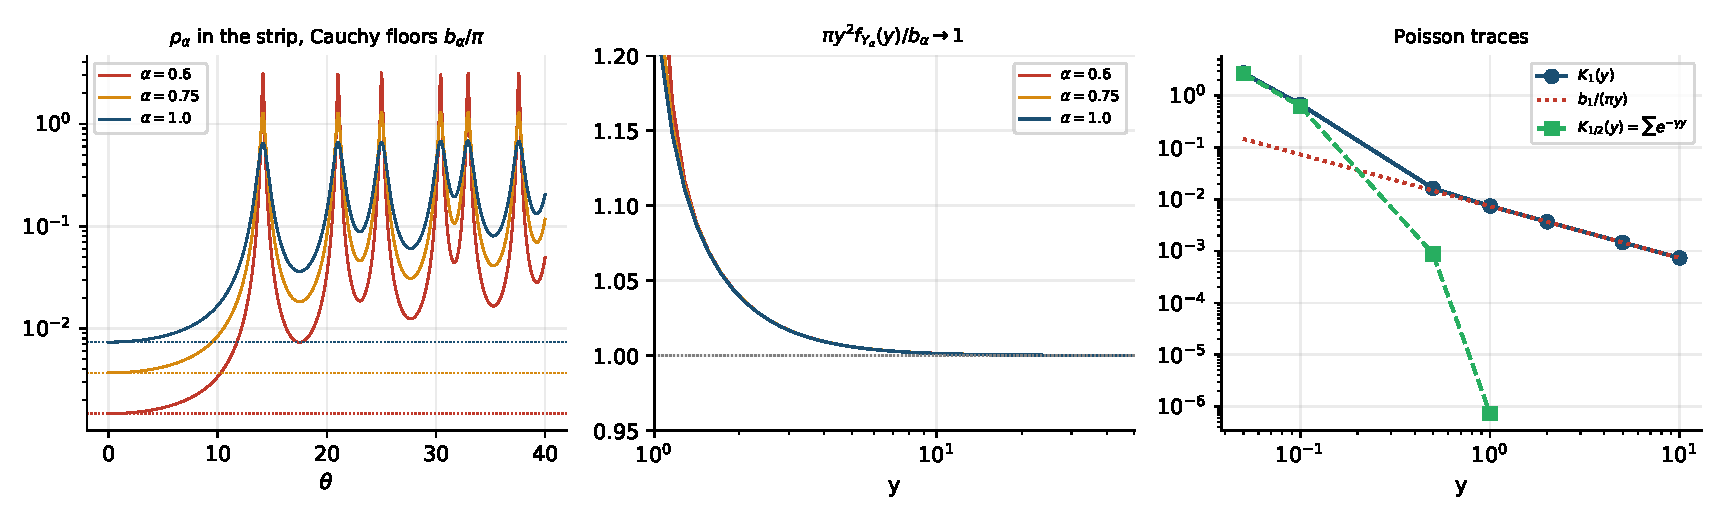
\includegraphics[width=\textwidth]{fig/bp1_strip.pdf}
\caption{Left: the Thorin densities $v_\alpha/\pi$ at $\alpha=0.6$, $0.75$, $1$, written $\rho_\alpha$ in the plot, and their Cauchy floors $b_\alpha/\pi$ (dotted). Middle: $\pi y^2f_{Y_\alpha}(y)/b_\alpha$, tending to one. Right: the Poisson traces $K_1$ and $K_{1/2}$ against $b_1/(\pi y)$. Drawn by \texttt{figs2.py} from \texttt{strip.json} and \texttt{comp.json}.}
\label{sm:fig:strip}
\end{figure}

Frullani's integral gives $\log(1+u^2/\theta^2)=\int_{\R}(1-\cos uy)\,e^{-\theta|y|}\frac{dy}{|y|}$, which is the sine squared lemma read in the other direction, since $1-\cos uy=2\sin^2(uy/2)$, and which is the cosine dictionary \eqref{rz:eq:cosdict} of Section~\ref{ch:rz2}. Inserting it in \eqref{sm:eq:thorin} puts the characteristic function of $Y_\alpha$ in L\'evy Khintchine form in $u$:
\begin{gather*}
\frac{\xi(\alpha)}{\xi(\alpha+|u|)}=\exp\Big\{-\int_{\R}2\sin^2\Big(\frac{uy}2\Big)\,\frac{K_\alpha(|y|)}{|y|}\,dy\Big\},\\
K_\alpha(y)=\frac1\pi\int_0^\infty e^{-\theta y}v_\alpha(\theta)\,d\theta .
\end{gather*}
So the L\'evy density of $Y_\alpha$ is $K_\alpha(|y|)/|y|$, as Section~\ref{sec:ch3:hierarchy} gives for a symmetric EGGC, and $K_\alpha$ is the Laplace transform of the Thorin density; in the normalisation of \eqref{rz:eq:cosdict}, $K_\alpha=\frac12K_{U_\alpha}$. We call $K_\alpha$ the Poisson trace, because at the centre, where under RH the Thorin measure in the chart $\theta$ is $\sum_{\gamma>0}\delta_\gamma$, it is $K_{1/2}(y)=\sum_{\gamma>0}e^{-\gamma y}$, half of Cram\'er's function \cite[Chapter I]{Cramer19} of Proposition~\ref{rz:prop:dict}(iii): the sum over the zeros of the Poisson kernel in place of the heat kernel of the heat trace $W(t)=\sum_ke^{-a_kt}$, which is $\sum_{\gamma>0}e^{-\gamma^2t}$ under RH. The two traces play parallel roles, and they are linked with no hypothesis. Since $Y_{1/2}=B_{2T}$ for an independent Brownian motion $B$, and $T$ has L\'evy density $W(t)/t$ (Theorem~\ref{thm:ch12:idsd}), the L\'evy density of $Y_{1/2}$ is $\int_0^\infty(4\pi t)^{-1/2}e^{-y^2/4t}\,W(t)\,t^{-1}dt$, so
\[
K_{1/2}(y)=\int_0^\infty\frac{y}{\sqrt{4\pi t^3}}\,e^{-y^2/4t}\,W(t)\,dt=\E\,W(H_{y/\sqrt2}),\qquad y>0 .
\]
The Poisson trace is the heat trace averaged over the first passage time of Brownian motion to the level $y/\sqrt2$, that is, subordinated by the stable one half first passage kernel, whose Laplace transform $e^{-y\sqrt a}$ is the stable one half average of the heat kernel recalled after Proposition~\ref{rz:prop:diverge}. This defines $K_{1/2}$ unconditionally, as $K_{1/2}(y)=\sum_ke^{-y\sqrt{a_k}}$ with the principal root, and makes it computable from the explicit formula \eqref{eq:ch2:Warith} for $W$; under RH the kernel integrates $e^{-\gamma^2t}$ to $e^{-\gamma y}$. Numerically, \texttt{improve.py} evaluates the integral with $W$ from the first $1700$ zeros and obtains $0.08566744234217$ at $y=0.2$ and $0.000883746148510$ at $y=0.5$, equal to $\sum e^{-\gamma y}$ over the same zeros to fourteen digits.

\begin{corollary}\label{sm:cor:poisson}
RH holds if and only if the Poisson trace $K_{1/2}$ is completely monotone, and if and only if the heat trace $W$ is completely monotone. For $\alpha\ge1$ the Poisson trace $K_\alpha$ is completely monotone with no hypothesis, and $K_\alpha(y)\sim b_\alpha/(\pi y)$ as $y\to\infty$, so that the L\'evy density of $Y_\alpha$ is asymptotic to $b_\alpha/(\pi y^2)$, the L\'evy density of the Cauchy component.
\end{corollary}

\begin{proof}
For $\alpha\ge1$, $K_\alpha$ is the Laplace transform of the positive density $v_\alpha/\pi$, hence completely monotone by Bernstein's theorem, and since $v_\alpha$ is continuous with $v_\alpha(0)=b_\alpha$, $yK_\alpha(y)\to b_\alpha/\pi$ as $y\to\infty$. At the centre, $W$ is completely monotone exactly when $T$ is a GGC (Section~\ref{ch:clock}), that is exactly when RH holds (Proposition~\ref{prop:rigid}). Under RH, $K_{1/2}(y)=\sum_{\gamma>0}e^{-\gamma y}$ is completely monotone. Conversely, suppose that $K_{1/2}(y)=\int_{[0,\infty)}e^{-y\theta}\nu(d\theta)$ with a positive measure $\nu$. For $w>0$ the unconditional formula $K_{1/2}(y)=\sum_ke^{-y\sqrt{a_k}}$ gives
\[
\int_0^\infty e^{-wy}\,y\,K_{1/2}(y)\,dy=\sum_k\frac1{(w+\sqrt{a_k})^2}=\int_{[0,\infty)}\frac{\nu(d\theta)}{(w+\theta)^2}.
\]
The first equality integrates term by term, which is legitimate because $\sqrt{a_k}=\gamma_k-i(\beta_k-\frac12)$ has real part $\gamma_k$ when $\rho_k=\beta_k+i\gamma_k$ is taken with $\gamma_k>0$, so the absolute values of the terms integrate to $\sum_k(w+\gamma_k)^{-2}<\infty$. The second is Tonelli's theorem, and it shows that the right side is finite for $w>0$. The middle expression is meromorphic in $w\in\C$, with a double pole at each point $-\sqrt{a_k}$, while the right side is holomorphic on $\cut$, since $|w+\theta|$ is bounded below by a positive multiple of $1+\theta$ for $w$ in a compact subset of $\cut$. The two sides agree for $w>0$, hence on $\cut$ with the poles removed, so no pole $-\sqrt{a_k}$ lies in $\cut$. Since $\re\sqrt{a_k}>0$, every $\sqrt{a_k}$ is therefore real and positive, that is, every $a_k=-(\rho_k-\frac12)^2$ is positive, which is RH.
\end{proof}

Table~\ref{sm:tab:K}, computed by \texttt{comp.py}, gives $K_1$ from $v_1$ on $[0,200]$ with the Weyl density beyond, and $K_{1/2}$ as $\sum e^{-\gamma y}$ over the first $1700$ zeros (Figure~\ref{sm:fig:strip}, right). At large $y$, $K_1(y)$ approaches $b_1/(\pi y)$, to $0.5\%$ at $y=10$, while $K_{1/2}(y)$ decays like $e^{-\gamma_1y}$: at the centre there is no Cauchy component, the tail is Laplace like with rate $\gamma_1$, and the variance is finite. At small $y$ both traces are large and close, because there the Poisson kernels see all zeros and the smoothing at the basepoint one matters little.

\begin{table}[htbp]
\centering\small
\begin{tabular}{cccc}
\toprule
$y$ & $K_1(y)=\frac1\pi\int_0^\infty e^{-\theta y}v_1(\theta)\,d\theta$ & $b_1/(\pi y)$ & $K_{1/2}(y)=\sum e^{-\gamma y}$\\
\midrule
0.05 & 2.7700 & 0.1470 & 2.6860\\
0.1 & 0.68408 & 0.07352 & 0.62104\\
0.5 & 0.016327 & 0.014703 & $8.84\times10^{-4}$\\
1 & 0.0074306 & 0.0073516 & $7.27\times10^{-7}$\\
2 & 0.0036856 & 0.0036758 & $5.28\times10^{-13}$\\
10 & 0.00073906 & 0.00073516 & $4.1\times10^{-62}$\\
\bottomrule
\end{tabular}
\caption{The Poisson traces at the basepoint one and at the centre, computed by \texttt{comp.py}.}
\label{sm:tab:K}
\end{table}

\subsection{The complete monotonicity conditions of the Poisson trace}\label{sec:biane:cm}

By Corollary~\ref{sm:cor:poisson}, RH is the complete monotonicity of the Poisson trace $K_{1/2}$. This subsection follows the first author's note on Biane's paper \cite{P26bia}. It writes the conditions out zero by zero, proves that a long initial stretch of them holds with no hypothesis, says which zeros each condition sees, gives two further equivalent forms, explains why the explicit formula cannot test the conditions, and compares $K_{1/2}$ with the corresponding trace of P\'olya's function $P(\theta)=K_{i\theta/2}(2\pi)$ of Section~\ref{ch:biane}, which is completely monotone with no hypothesis. The computations are in \texttt{biane\_traces.py} and \texttt{biane\_figs.py}.

Write the zeros as $\rho_k=\beta_k+i\gamma_k$ with $\gamma_k>0$, so that $\sqrt{a_k}=\gamma_k+i\delta_k$ with $\delta_k=\frac12-\beta_k\in(-\frac12,\frac12)$, and put $\varphi_k=\arctan(\delta_k/\gamma_k)$. The series $K_{1/2}(y)=\sum_ke^{-y\sqrt{a_k}}$ converges absolutely, with all its derivatives, for $y>0$, and the zeros $\rho_k$ and $1-\bar\rho_k$ have conjugate values of $\sqrt{a_k}$. Hence
\begin{equation}\label{eq:biane:cmcond}
(-1)^nK_{1/2}^{(n)}(y)=\sum_k\re\big((\sqrt{a_k})^ne^{-y\sqrt{a_k}}\big)=\sum_k|\sqrt{a_k}|^n\,e^{-\gamma_ky}\cos(n\varphi_k-\delta_ky),
\end{equation}
with each zero counted once, with its multiplicity; a zero on the line contributes $\gamma_k^ne^{-\gamma_ky}>0$. The note \cite{P26bia} groups $\rho_k$ with $1-\bar\rho_k$ and writes a factor $2$ in front of every term, which counts the zeros on the line twice. So $K_{1/2}$ is completely monotone, and by Corollary~\ref{sm:cor:poisson} RH holds, exactly when every one of the quantities \eqref{eq:biane:cmcond} is nonnegative, for $n=0,1,2,\dots$ and $y>0$. Off the line a term oscillates in $n$ with the small frequency $\varphi_k\approx\delta_k/\gamma_k$, so a zero off the line can spoil its term only at a high order.

\begin{proposition}\label{prop:biane:termwise}
The term of a zero with $\delta_k\ne0$ in \eqref{eq:biane:cmcond} is positive whenever
\[
n\arctan\frac{|\delta_k|}{\gamma_k}+|\delta_k|\,y<\frac\pi2 .
\]
If $\delta_k>0$ and $\delta_ky<\frac\pi2$, the first order $n$ at which the term is negative is the least integer with $n\varphi_k-\delta_ky>\frac\pi2$, that is the least integer above $(\frac\pi2+\delta_ky)/\varphi_k$ when this ratio is not an integer. The partner $1-\bar\rho_k$ has the same term.
\end{proposition}

\begin{proof}
$|n\varphi_k-\delta_ky|\le n|\varphi_k|+|\delta_k|y$, and the cosine is positive on $(-\frac\pi2,\frac\pi2)$. For $\delta_k>0$ the argument $n\varphi_k-\delta_ky$ increases with $n$ from $-\delta_ky\in(-\frac\pi2,0)$, and the cosine is first negative when it passes $\frac\pi2$. The partner has $-\delta_k$ and $-\varphi_k$, so its argument is the negative of this one.
\end{proof}

\texttt{biane\_traces.py} finds the first negative order by evaluating the sign factor; Table~\ref{tab:biane:cmorders} compares it with the formula, and the note's values are the same.

\begin{table}[htbp]
\centering\small
\begin{tabular}{rrrrr}
\toprule
$\gamma$ & $\delta$ & $y$ & first negative order & $(\frac\pi2+\delta y)/\varphi$\\
\midrule
$50$ & $0.25$ & $1$ & $365$ & $364.16$\\
$50$ & $0.25$ & $0.3$ & $330$ & $329.16$\\
$200$ & $0.1$ & $1$ & $3342$ & $3341.59$\\
$14.13$ & $0.5$ & $0.5$ & $52$ & $51.48$\\
\bottomrule
\end{tabular}
\caption{The first order at which the term of a hypothetical zero $\frac12-\delta+i\gamma$ in \eqref{eq:biane:cmcond} is negative, against Proposition~\ref{prop:biane:termwise}. The last row is a zero at the edge of the strip at the height of the first ordinate. Computed by \texttt{biane\_traces.py}.}
\label{tab:biane:cmorders}
\end{table}

\begin{theorem}\label{thm:biane:cmrange}
Suppose that every zero with $0<\gamma_k\le H$ lies on the critical line. Then for $0<y<\pi$ and every integer $n$ with $0\le n<H(\pi-y)$, every term of \eqref{eq:biane:cmcond} is positive, and $(-1)^nK_{1/2}^{(n)}(y)>0$. With $H=T_0=3\times10^{12}$ \cite{PT21} this covers all $n<9.12\times10^{12}$ at $y=0.1$, $n<6.42\times10^{12}$ at $y=1$ and $n<4.24\times10^{11}$ at $y=3$.
\end{theorem}

\begin{proof}
A zero with $\gamma_k\le H$ has $\delta_k=0$, and its term $\gamma_k^ne^{-\gamma_ky}$ is positive. A zero with $\gamma_k>H$ has $|\varphi_k|\le|\delta_k|/\gamma_k<\frac1{2H}$ and $|\delta_k|y<\frac y2$, so $n|\varphi_k|+|\delta_k|y<\frac n{2H}+\frac y2\le\frac\pi2$ when $n\le H(\pi-y)$, and its term is positive by Proposition~\ref{prop:biane:termwise}. The series converges absolutely, so its sum is positive.
\end{proof}

The theorem is a statement about the verified height, not about $K_{1/2}$: it improves with every extension of the verification and never reaches the whole family. Every condition that could fail has $y\ge\pi$ or $n\ge H(\pi-y)$, which is above $4\times10^{11}$ for $y\le3$; there, complete monotonicity is a characterisation of RH, not a test that a computation could run to a failure. The note \cite{P26bia} gives the last bound as $4.3\times10^{11}$; it is $4.2478\times10^{11}$.

The weight of the zero $\gamma_k$ in the condition $(n,y)$ is about $\gamma_k^ne^{-\gamma_ky}$, whose logarithm $n\log\gamma-\gamma y$ is largest at
\[
\gamma_*=\frac ny,
\]
with a width of order $\sqrt n/y$. The condition $(n,y)$ is therefore a smoothed probe of the zeros near the height $n/y$. Among the first $300$ ordinates the dominant one is $21.022$ for $(n,y)=(20,1)$, $98.831$ for $(100,1)$ and for $(50,0.5)$, with $101.318$ a close second (the logarithms of the weights at $(100,1)$ are $360.51013$ and $360.50841$), $21.022$ for $(100,5)$ and $30.425$ for $(300,10)$: in each case the ordinate nearest to $n/y$ (\texttt{biane\_traces.py}). Figure~\ref{fig:biane:cm} shows two weight profiles and two sign factors. The reading explains Theorem~\ref{thm:biane:cmrange} and shows its edge. By Proposition~\ref{prop:biane:termwise} a zero at height $\gamma$ can make its term negative only when $n\gtrsim\frac\pi2\gamma/|\delta|\ge\pi\gamma$, that is when $\gamma\lesssim n/\pi$, below the peak at $n/y$ when $y<\pi$; and since $\gamma^ne^{-\gamma y}$ increases up to $n/y$, its value at $\gamma\le n/\pi$ is at most $\exp(n(\log\frac y\pi+1-\frac y\pi))$ times its value at the peak, which is exponentially small in $n$. Turning this comparison into a proof would need a bound for the number of zeros off the line near each height, and it would push the unconditional range beyond $H(\pi-y)$ without reaching the whole family: the conditions with $n/y$ beyond every verified height are the content of RH.

\begin{figure}[htbp]
\centering
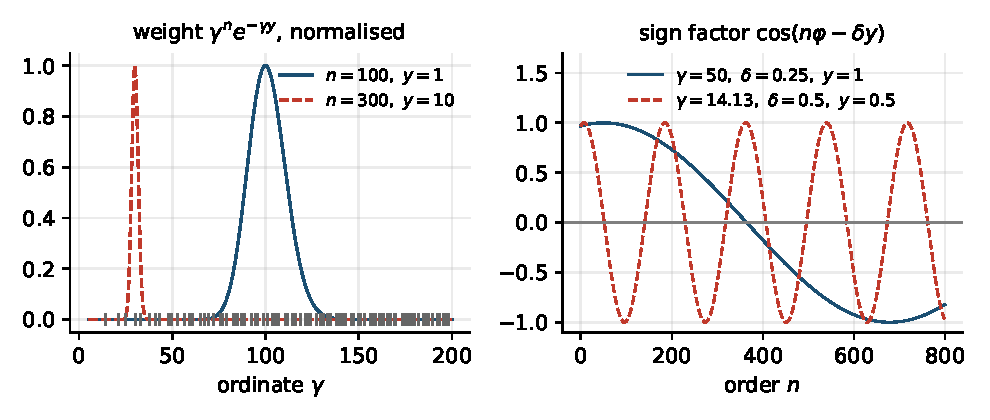
\includegraphics[width=\textwidth]{fig/biane_cm.pdf}
\caption{Left: the weight $\gamma^ne^{-\gamma y}$ of the condition $(n,y)$ in \eqref{eq:biane:cmcond}, normalised to maximum one, for $(n,y)=(100,1)$ and $(300,10)$, peaking at $\gamma=n/y$; the marks are the ordinates below $200$. Right: the sign factor $\cos(n\varphi-\delta y)$ of a hypothetical zero off the line for $(\gamma,\delta,y)=(50,0.25,1)$ and $(14.13,0.5,0.5)$, positive below the orders $365$ and $52$ of Table~\ref{tab:biane:cmorders}, at which it is first negative. Drawn by \texttt{biane\_figs.py} from \texttt{biane\_traces.json}.}
\label{fig:biane:cm}
\end{figure}

\begin{proposition}\label{prop:biane:pd}
The following are equivalent:
\begin{enumerate}
\item[(i)] RH;
\item[(ii)] $K_{1/2}$ is completely monotone on $(0,\infty)$;
\item[(iii)] for every $x>0$ the function $y\mapsto K_{1/2}(x+iy)$ is positive definite on $\R$;
\item[(iv)] for some $x>0$ the function $y\mapsto K_{1/2}(x+iy)$ is bounded on $[0,\infty)$.
\end{enumerate}
Under these conditions $|K_{1/2}(x+iy)|\le K_{1/2}(x)$.
\end{proposition}

\begin{proof}
The series $K_{1/2}(z)=\sum_ke^{-z\sqrt{a_k}}$ converges absolutely and locally uniformly for $\re z>0$, since $|e^{-z\sqrt{a_k}}|=e^{-\gamma_k\re z+\delta_k\im z}\le e^{-\gamma_k\re z+|\im z|/2}$, and defines an analytic function there. (i) implies (ii) by Corollary~\ref{sm:cor:poisson}. If (ii) holds, Bernstein's theorem gives $K_{1/2}(y)=\int_{[0,\infty)}e^{-y\theta}\nu(d\theta)$ with a positive measure $\nu$, the integral converges for $\re z>0$ and agrees there with $K_{1/2}(z)$ by analytic continuation, and $K_{1/2}(x+iy)=\int e^{-iy\theta}e^{-x\theta}\nu(d\theta)$ is the Fourier transform of the finite positive measure $e^{-x\theta}\nu(d\theta)$, which gives (iii) and the bound. A positive definite function $f$ satisfies $|f(y)|\le f(0)$, so (iii) implies (iv). Suppose (iv) holds at $x$. For $\re w>\frac12$ the bound above allows term by term integration, and
\[
\int_0^\infty e^{-wy}K_{1/2}(x+iy)\,dy=\sum_k\frac{e^{-x\sqrt{a_k}}}{w+i\sqrt{a_k}} .
\]
The right side is a meromorphic function of $w\in\C$, since $\sum_ke^{-x\gamma_k}<\infty$, with a pole at each point $-i\sqrt{a_k}=\delta_k-i\gamma_k$, of residue $e^{-x\sqrt{a_k}}$ times the multiplicity, which is not zero. Since $K_{1/2}(x+iy)$ is bounded, the left side is analytic in $\re w>0$, so no pole has $\delta_k>0$. The zeros $\rho_k$ and $1-\bar\rho_k$ have opposite $\delta_k$, so every $\delta_k$ is $0$, which is RH.
\end{proof}

Part (iv) replaces the Paley Wiener argument of the note \cite{P26bia}, which is not given in detail there, by a pole of a Laplace transform. Written out, (iii) says that for every $x>0$, all real $y_1,\dots,y_m$ and all complex $c_1,\dots,c_m$,
\[
\sum_{j,l}c_j\bar c_l\,K_{1/2}\big(x+i(y_j-y_l)\big)=\sum_ke^{-x\gamma_k}\Big|\sum_jc_je^{-i\gamma_ky_j}\Big|^2\ge0,
\]
the equality holding under RH. This is a positivity of the kind in Weil's criterion, with two differences: the test functions are $r\mapsto e^{-rx}|\sum_jc_je^{-iry_j}|^2$ on $r>0$, where the damping $e^{-rx}$ does the work of a decay hypothesis, and the sum runs over the ordinates in the upper half plane only.

One would like to turn each condition into a statement about primes with the explicit formula of Section~\ref{ch:clock}, the display before \eqref{eq:ch2:Warith}. The test function of the condition $(n,y)$ is $h(r)=|r|^ne^{-y|r|}$, with
\[
g(x)=\frac1{2\pi}\int_{\R}h(r)e^{-irx}\,dr=\frac{n!}\pi\re\frac1{(y+ix)^{n+1}},
\]
which decays only like a power of $|x|$ and has one sign for large $|x|$. The prime side $-2\sum_{m\ge2}\Lambda(m)m^{-1/2}g(\log m)$ then diverges, since $\sum_pp^{-1/2}(\log p)^{-j}=\infty$ for every $j$; the formula holds for $g$ decaying faster than $e^{-|x|/2}$, which goes with $h$ analytic in a strip $|\im r|<\frac12+\epsilon$, and this $h$ is not even analytic at $r=0$. For $n=0$ the prime side is $-\frac2\pi\sum_{m\ge2}\Lambda(m)m^{-1/2}y/(y^2+\log^2m)$, which is what the prime terms of \eqref{eq:ch2:Warith} become under the subordination $K_{1/2}(y)=\E W(H_{y/\sqrt2})$ of Section~\ref{sm:sec:poisson}, applied term by term, with twice $K_{1/2}$ on the left; its terms have poles at $y=\pm i\log m$, the singularities of Cram\'er's function \cite[Chapter I]{Cramer19}, and it diverges for the reason of Proposition~\ref{rz:prop:diverge}. Smoothing in the variable of the zeros removes the divergence without changing the problem: the Gaussian weight $e^{-r^2t}$ in place of $e^{-y|r|}$ gives the heat trace $W(t)$, whose explicit formula \eqref{eq:ch2:Warith} converges absolutely, and whose complete monotonicity is again equivalent to RH (Corollary~\ref{sm:cor:poisson}). The note \cite{P26bia} identifies this smoothing with the de Bruijn Newman flow and concludes that the primes become summable only at times $t>0$, where the reality of the zeros is known; but the Gaussian weight acts on the test function, while the flow multiplies the kernel $\Phi$ by $e^{tu^2/4}$ and moves the zeros, and the smoothed conditions, those of the heat trace, are still equivalent to RH.

The last comparison is with P\'olya's function. By Proposition~\ref{prop:biane:sin2},
\begin{gather*}
\log\frac{K_{\lambda/2}(2\pi)}{K_0(2\pi)}=\int_0^\infty4\sin^2\Big(\frac{\lambda y}2\Big)K^P(y)\,\frac{dy}y,\\
K^P(y)=\sum_ne^{-2\nu_ny}=\operatorname{tr}e^{-2y\sqrt{A_P}},
\end{gather*}
the sum over the zeros $\theta_n=2\nu_n$ of $P$, so $K^P$ is the counterpart of $K_{1/2}$ in the formula for $\xi(\frac12)/\xi(\frac12+u)$, and it is completely monotone because $A_P$ is selfadjoint and positive. By Proposition~\ref{prop:biane:phase} the two traces have the same main term, and their difference has a limit.

\begin{proposition}\label{prop:biane:traces}
Let $M(y)=\frac1{2\pi y}\big(\log\frac1{2\pi y}-\gamma_E\big)$ and $c=2\pi-\frac1{6\pi}-\frac1{48\pi}=6.2235022035$. As $y\to0+$:
\begin{enumerate}
\item[(i)] $K_{1/2}(y)=M(y)+\frac78+O(y\log\frac1y)$, and under RH $K_{1/2}(y)=M(y)+\frac78+\frac1{48\pi}y\log\frac1y+o(y\log\frac1y)$;
\item[(ii)] $K^P(y)=M(y)-\frac14+\big(2\pi-\frac1{6\pi}\big)y\log\frac1y+O(y)$;
\item[(iii)] $D(y)=K_{1/2}(y)-K^P(y)=\frac98+O(y\log\frac1y)$, and under RH $D(y)=\frac98-c\,y\log\frac1y+o(y\log\frac1y)$.
\end{enumerate}
\end{proposition}

\begin{proof}
(i) The real part of the term $e^{-y\sqrt{a_k}}$ is $e^{-\gamma_ky}\cos(\delta_ky)=e^{-\gamma_ky}+O(y^2e^{-\gamma_ky})$, and the imaginary parts cancel in pairs, so $K_{1/2}(y)=\sum_ke^{-\gamma_ky}+O(y^2\sum_ke^{-\gamma_ky})$, and the sum will turn out to be $O(y^{-1}\log\frac1y)$. By Abel summation $\sum_ke^{-\gamma_ky}=y\int_0^\infty e^{-Ty}N(T)\,dT$, with $N(T)=\vartheta(T)/\pi+1+S(T)$ \cite[Section 9.3]{Titchmarsh}. The Riemann Siegel function satisfies $\vartheta(T)/\pi=N_0(T)-\frac18+\frac1{48\pi T}+O(T^{-3})$ with $N_0(T)=\frac T{2\pi}\log\frac T{2\pi e}$, so $N=N_0+\frac78+S+E$ with $E(T)=\frac1{48\pi T}+O(T^{-3})$ for $T\ge1$ and $E$ bounded on $(0,1]$. Now $\int_0^\infty Te^{-Ty}\log T\,dT=y^{-2}(1-\gamma_E-\log y)$ gives $y\int_0^\infty e^{-Ty}N_0(T)\,dT=M(y)$; the constant gives $\frac78$; $y\int_1^\infty e^{-Ty}\frac{dT}{48\pi T}=\frac1{48\pi}y\log\frac1y+O(y)$, and the rest of $E$ gives $O(y)$. With $S_1(T)=\int_0^TS(t)\,dt$, an integration by parts gives $y\int_0^\infty e^{-Ty}S(T)\,dT=y^2\int_0^\infty e^{-Ty}S_1(T)\,dT$, which is $O(y\log\frac1y)$ since $S_1(T)=O(\log T)$ \cite[Theorem 9.9(A)]{Titchmarsh}. Under RH there are no terms $O(y^2e^{-\gamma_ky})$, and $S_1(T)=O(\log T/(\log\log T)^2)$ \cite[Theorem 14.13]{Titchmarsh} makes the last integral $o(y\log\frac1y)$. (ii) By Proposition~\ref{prop:biane:phase}, the number of zeros $\theta_n\le T$ is $\lfloor x(T)\rfloor$, with $x(T)=N_0(T)+\frac14+(2\pi-\frac1{6\pi})T^{-1}+O(T^{-3})$ for $T\ge1$. Write $\lfloor x\rfloor=x-\frac12+(\frac12-\{x\})$. The terms $N_0$, $\frac14-\frac12$ and $(2\pi-\frac1{6\pi})T^{-1}$ give $M(y)$, $-\frac14$ and $(2\pi-\frac1{6\pi})y\log\frac1y+O(y)$ as in (i). The sawtooth $\frac12-\{x(T)\}$ has integral over each interval on which $x$ increases by one equal to $O(T^{-1}(\log T)^{-3})$, because such an interval has length about $2\pi/\log T$ and $x'(T)=\frac1{2\pi}\log\frac T{2\pi}+O(T^{-2})$ varies over it by $O(T^{-1}(\log T)^{-2})$ relative to its size, so its integral from $0$ to $T$ is bounded, and another integration by parts makes its contribution $O(y)$. (iii) is (i) minus (ii).
\end{proof}

\texttt{biane\_traces.py} tests the proposition. It takes the first $30000$ ordinates from Arb, up to $25755.348$, cuts at $G=25754.905$, midway between the last two, and adds the tail $\int_G^\infty e^{-Ty}\vartheta'(T)\,dT/\pi-e^{-Gy}S(G)$, with $S(G)=-0.569$ exact; the neglected term $y\int_G^\infty e^{-Ty}S(T)\,dT$ equals $y^2\int_G^\infty e^{-Ty}\int_G^TS(t)\,dt\,dT$, and Trudgian's bound $|\int_{t_1}^{t_2}S(t)\,dt|\le2.067+0.059\log t_2$ for $t_2>t_1>168\pi$ \cite{Trudgian11}, with Jensen's inequality for the logarithm, bounds it by $ye^{-Gy}(0.059\log(G+1/y)+2.067)$; the script records twice this bound, $3.5\times10^{-14}$, $4.1\times10^{-5}$ and $4.3\times10^{-5}$ at $y=10^{-3}$, $10^{-4}$ and $10^{-5}$, so the entries of Table~\ref{tab:biane:traces} at $y=10^{-4}$ and $10^{-5}$ may be off by up to two units in the fifth decimal. The zeros of $P$ come from the phase condition of Proposition~\ref{prop:biane:phase}, solved by Newton's method for all $30132$ zeros to just above the cut, with phase residuals below $4.4\times10^{-11}$; the $29998$ below $G$ are summed and the tail $\int_G^\infty e^{-Ty}\,dx(T)+e^{-Gy}(\{x(G)\}-\frac12)$ is added, with $x(G)=29998.944$. The factor $e^{-Gy}$ that weights the tails is $2.6\times10^{-6}$ at $y=5\times10^{-4}$, $0.0058$ at $2\times10^{-4}$, $0.076$ at $10^{-4}$ and $0.77$ at $10^{-5}$, so the last row of Table~\ref{tab:biane:traces} rests mostly on the smooth tails. The constant $\frac98$ appears clearly, and $D$ approaches it along $\frac98-cy\log\frac1y$ (Figure~\ref{fig:biane:traces}).

\begin{table}[htbp]
\centering\small
\fitwidth{\begin{tabular}{lrrrrrr}
\toprule
$y$ & $K_{1/2}(y)$ & $K^P(y)$ & $K_{1/2}-M$ & $K^P-M$ & $D(y)$ & $\frac98-cy\log\frac1y$\\
\midrule
$0.05$ & $2.686015$ & $2.230883$ & $0.837782$ & $0.382650$ & $0.455132$ & $0.192803$\\
$0.02$ & $12.772471$ & $12.033884$ & $0.860279$ & $0.121691$ & $0.738587$ & $0.638070$\\
$0.01$ & $35.723862$ & $34.836495$ & $0.867696$ & $-0.019670$ & $0.887366$ & $0.838397$\\
$0.005$ & $92.647265$ & $91.663043$ & $0.871374$ & $-0.112848$ & $0.984222$ & $0.960130$\\
$0.003$ & $180.932794$ & $179.901902$ & $0.872836$ & $-0.158057$ & $1.030892$ & $1.016540$\\
$0.002$ & $303.229389$ & $302.172210$ & $0.873563$ & $-0.183616$ & $1.057179$ & $1.047647$\\
$0.001$ & $715.903738$ & $714.816981$ & $0.874286$ & $-0.212471$ & $1.086757$ & $1.082010$\\
$5\times10^{-4}$ & $1651.569150$ & $1650.465433$ & $0.874645$ & $-0.229071$ & $1.103717$ & $1.101348$\\
$2\times10^{-4}$ & $4856.772117$ & $4855.656772$ & $0.874859$ & $-0.240486$ & $1.115345$ & $1.114399$\\
$10^{-4}$ & $10815.847446$ & $10814.727704$ & $0.874931$ & $-0.244811$ & $1.119742$ & $1.119268$\\
$10^{-5}$ & $144797.380092$ & $144796.255761$ & $0.874994$ & $-0.249338$ & $1.124332$ & $1.124283$\\
\bottomrule
\end{tabular}}
\caption{The Poisson trace $K_{1/2}$ of the zeros of $\zeta$, P\'olya's trace $K^P$, their distances from the common main term $M$, which tend to $\frac78$ and $-\frac14$, and their difference $D$, which tends to $\frac98$, against the prediction of Proposition~\ref{prop:biane:traces} under RH. Computed by \texttt{biane\_traces.py}.}
\label{tab:biane:traces}
\end{table}

\begin{figure}[htbp]
\centering
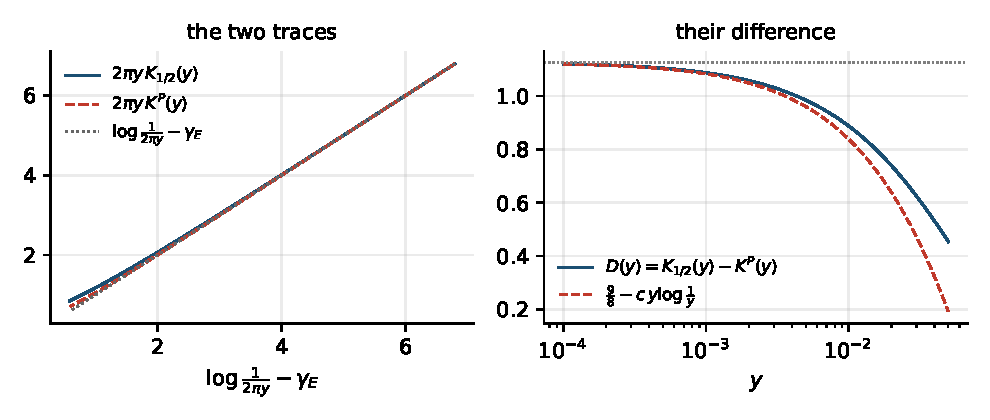
\includegraphics[width=\textwidth]{fig/biane_traces.pdf}
\caption{Left: $2\pi yK_{1/2}(y)$ and $2\pi yK^P(y)$ against $\log\frac1{2\pi y}-\gamma_E$ for $10^{-4}\le y\le0.05$, with the main term $2\pi yM(y)$ (dotted). Right: the difference $D(y)$, the limit $\frac98$ (dotted) and $\frac98-cy\log\frac1y$ (dashed). Drawn by \texttt{biane\_figs.py} from \texttt{biane\_traces.json}.}
\label{fig:biane:traces}
\end{figure}

The note \cite{P26bia} states that $K_{1/2}(y)=M(y)+O(\log\frac1y)$, which is true but loses the constant, and it reports $D(y)/\log\frac1y=0.195$, $0.194$, $0.193$, $0.193$ at $y=0.003$, $0.005$, $0.01$, $0.02$, from which it concludes that $D$ grows like $0.19\log\frac1y$. Repeating its computation, with the first $300$ ordinates and the $312$ zeros of $P$ below $\gamma_{300}+20=561.85$, each followed by a plain Weyl tail from the last zero, gives its ratios $K_{1/2}/M=1.0059$, $1.0102$, $1.0250$, $1.0722$ and $D/\log\frac1y=0.195$, $0.192$, $0.193$, $0.189$; the note describes the $312$ zeros as lying below $\gamma_{300}=541.85$, below which there are $298$. The accurate values of $D/\log\frac1y$ in this range, $0.177$, $0.186$, $0.193$, $0.189$, are also close to $0.19$, but that is a coincidence of the range: by Proposition~\ref{prop:biane:traces}, $D$ tends to $\frac98$, and $D/\log\frac1y$ is $0.098$ at $y=10^{-5}$.

The comparison shows where the difficulty sits. $K^P$ is completely monotone for a structural reason, as the trace of the semigroup $e^{-2y\sqrt{A_P}}$. By Corollary~\ref{sm:cor:poisson}, RH says that $K_{1/2}=K^P+D$ is completely monotone as well, where $D$ is bounded, tends to $\frac98$ while both traces grow like $\frac1{2\pi y}\log\frac1y$, and carries the whole difference between $\Phi$ and P\'olya's kernel, the arithmetic included. Complete monotonicity constrains the derivatives of every order, and no bound on the size of $D$ can decide it.

\subsection{Wiener's theorem and the basepoint kernels}\label{wr:sec:wiener}

The zero free half planes that recur through Chapter~\ref{chap:basepoint} and through Sections~\ref{sm:sec:cf} to \ref{sm:sec:poisson} have a second reading, as completeness statements, through Wiener's closure theorem \cite{Wiener32}, for which Kac \cite{Kac65} and Korevaar \cite{Korevaar65} gave short alternative treatments: the translates $f(\cdot-x)$, $x\in\R$, of a function $f\in L^1(\R)$ span a dense subspace of $L^1(\R)$ if and only if its Fourier transform $\hat f(\theta)=\int f(u)e^{i\theta u}du$ has no real zeros. The $L^2$ version asks only that $\hat f\ne0$ almost everywhere; since the zeros of $\xi$ are isolated it never sees them, and it is the $L^1$ version that is sharp here.

Let $\Phi$ be P\'olya's kernel \eqref{eq:ch2:Phi}, so that $\xi(\frac12+s)=\int_{\R}\Phi(u)e^{su}du$ for every complex $s$ by \eqref{eq:ch2:mgf}, and for $\alpha\ge\frac12$ put
\begin{equation}\label{wr:eq:kernel}
\Phi_\alpha(u)=e^{(\alpha-\frac12)u}\,\Phi(u),\qquad \hat\Phi_\alpha(\theta)=\int_{\R}\Phi_\alpha(u)e^{i\theta u}du=\xi(\alpha+i\theta).
\end{equation}
Up to the factor $\xi(\alpha)$, $\Phi_\alpha$ is the density of the tilted P\'olya variable $V_\alpha$ of Section~\ref{bp:sec:mellin}, with $\E e^{sV_\alpha}=\xi(\alpha+s)/\xi(\alpha)$, and it is integrable for every $\alpha$ because $\Phi$ decays doubly exponentially. The real zeros of $\hat\Phi_\alpha$ are exactly the ordinates of the zeros of $\zeta$ on the line $\re s=\alpha$, so Wiener's theorem gives the following.

\begin{proposition}\label{wr:prop:wiener}
\begin{enumerate}
\item The translates of $\Phi_\alpha$ are dense in $L^1(\R)$ if and only if $\zeta$ has no zeros on the line $\re s=\alpha$.
\item At the centre they are not dense. For every finite combination $h=\sum_kc_k\Phi(\cdot-x_k)$ and every $g\in L^1(\R)$,
\[
\|g-h\|_1\ \ge\ \sup_\gamma|\hat g(\gamma)|,
\]
the supremum over the ordinates of the zeros on the critical line.
\item At the basepoint one they are dense, with no hypothesis, because $\xi(1+i\theta)\ne0$.
\item For $\alpha_0\in[\frac12,1)$, $\zeta$ has no zeros in the half plane $\re s>\alpha_0$ if and only if the translates of $\Phi_\alpha$ are dense in $L^1(\R)$ for every $\alpha>\alpha_0$. In particular RH holds if and only if they are dense for every $\alpha>\frac12$.
\item If the translates of $\Phi_\alpha$ are dense, approximation near the zeros is expensive: if $h=\sum_kc_k\Phi_\alpha(\cdot-x_k)$ and $\|g-h\|_1\le\delta$, then $\sum_k|c_k|\ \ge\ (|\hat g(\gamma)|-\delta)/|\xi(\alpha+i\gamma)|$ for every ordinate $\gamma$.
\end{enumerate}
\end{proposition}

\begin{proof}
(1), (3) and (4) are Wiener's theorem applied to $\hat\Phi_\alpha(\theta)=\xi(\alpha+i\theta)$, together with the nonvanishing of $\zeta$ on the line $\re s=1$. For (2) and (5), $\hat h(\theta)=\hat\Phi_\alpha(\theta)\sum_kc_ke^{i\theta x_k}$, so at the centre $\hat h(\gamma)=0$ at every ordinate of a zero on the line, while $|\hat g(\theta)-\hat h(\theta)|\le\|g-h\|_1$ for every $\theta$; for (5), $|\hat h(\gamma)|\le|\xi(\alpha+i\gamma)|\sum_k|c_k|$.
\end{proof}

Wiener's proof of the prime number theorem runs through statement (3), and the proposition shows the whole family interpolating between that theorem at $\alpha=1$ and RH at $\alpha=\frac12$. It is a restatement rather than a new criterion. By statement (4), completeness at every $\alpha'>\alpha$ is the absence of zeros with real part greater than $\alpha$. That is the condition $\alpha\ge\sup_\rho\re\rho$ under which $T_\alpha$ is a GGC (Theorem~\ref{thm:poisson}) and $Y_\alpha$ an EGGC (Theorem~\ref{sm:thm:thorin}), and, by Lagarias's argument \cite{Lagarias}, it is also the positivity of $v_{\alpha'}$ for every $\alpha'>\alpha$ (Remark~\ref{rem:ch2:oneline}). A zero exactly on the line $\re s=\alpha$ is allowed by the GGC property, and contributes an atom to the Thorin measure, but it blocks completeness at $\alpha$ itself; and for $\xi$ it is not known whether positivity of $v_\alpha$ on the single line $\re s=\alpha$ excludes zeros to its right (Exercise~\ref{ex:ch2:line}). What the completeness form adds is an explicit, computable obstruction at the centre, statement (2), and an explicit cost of approximation above it, statement (5): near the centre $|\xi(\alpha+i\gamma)|\approx(\alpha-\frac12)|\xi'(\frac12+i\gamma)|$ at the ordinate $\gamma$ of a simple zero, so the coefficients needed to reproduce $\hat g$ at an ordinate grow like $1/(\alpha-\frac12)$. At the first ordinate $|\xi'(\frac12+i\gamma_1)|=0.00138272$, and $|\xi(\alpha+i\gamma_1)|=0.000138$, $0.000346$, $0.000697$ at $\alpha=0.6$, $0.75$, $1$, as computed by \texttt{wiener.py}.

We tested the dichotomy with \texttt{wiener.py}. We approximated the Gaussian $g(u)=(2\pi\kappa^2)^{-1/2}e^{-u^2/2\kappa^2}$ with $\kappa=0.15$, for which $\hat g(\gamma_1)=e^{-\kappa^2\gamma_1^2/2}=0.10565$, by combinations of $N$ equally spaced translates of $\Phi_\alpha$ on $[-1.5,1.5]$, minimising the $L^1$ error on $[-3,3]$ exactly by linear programming. Table~\ref{wr:tab:wiener} and Figure~\ref{wr:fig:wiener} show the results. At the centre every approximant has $\hat h(\gamma_1)=0$ up to rounding, the computed values staying below $1.2\times10^{-8}$ while the coefficient sums grow to $4\times10^9$, and the best error stalls at $0.1345$, above the barrier $0.1056$ of statement (2), however many translates are used. Above the centre the error falls below the value at which the centre stalls and keeps decreasing, to below the barrier at $\alpha=0.75$ and $\alpha=1$; the barrier binds only at the centre, and at $\alpha=0.6$ the error is still $0.1139$ with $80$ translates. The approximants acquire the missing Fourier mass at $\gamma_1$: $|\hat h(\gamma_1)|$ reaches $0.017$, $0.038$ and $0.063$ at $\alpha=0.6$, $0.75$ and $1$ with $80$ translates, against the target $0.106$. The remaining error is limited by conditioning rather than by completeness. With $80$ translates the coefficient sums reach $3\times10^7$ to $2\times10^8$ above the centre, as statement (5) and the rapid decay of $\hat\Phi_\alpha$ require, and double precision linear programming cannot go much further. The experiment therefore shows the qualitative dichotomy clearly and the rate only roughly; the closer $\alpha$ is to $\frac12$, the larger the coefficients and the slower the approach, which is the completeness counterpart of the Cauchy kernels sharpening onto the zeros.

\begin{table}[htbp]
\centering\small
\begin{tabular}{ccccc}
\toprule
$N$ & $\alpha=\frac12$ & $\alpha=0.6$ & $\alpha=0.75$ & $\alpha=1$\\
\midrule
10 & 0.4705 & 0.4698 & 0.4664 & 0.4540\\
20 & 0.1345 & 0.1221 & 0.1060 & 0.0852\\
40 & 0.1345 & 0.1152 & 0.0907 & 0.0614\\
80 & 0.1365 & 0.1139 & 0.0878 & 0.0570\\
\midrule
$|\hat h(\gamma_1)|$ at $N=80$ & $0$ & 0.0167 & 0.0377 & 0.0635\\
\bottomrule
\end{tabular}
\caption{Best $L^1$ error in approximating a Gaussian of width $0.15$ by $N$ translates of $\Phi_\alpha$, computed by \texttt{wiener.py}. At the centre the error cannot fall below $|\hat g(\gamma_1)|=0.1056$, and $\hat h(\gamma_1)$ vanishes exactly; the computed value is $1.2\times10^{-8}$.}
\label{wr:tab:wiener}
\end{table}

\begin{figure}[htbp]
\centering
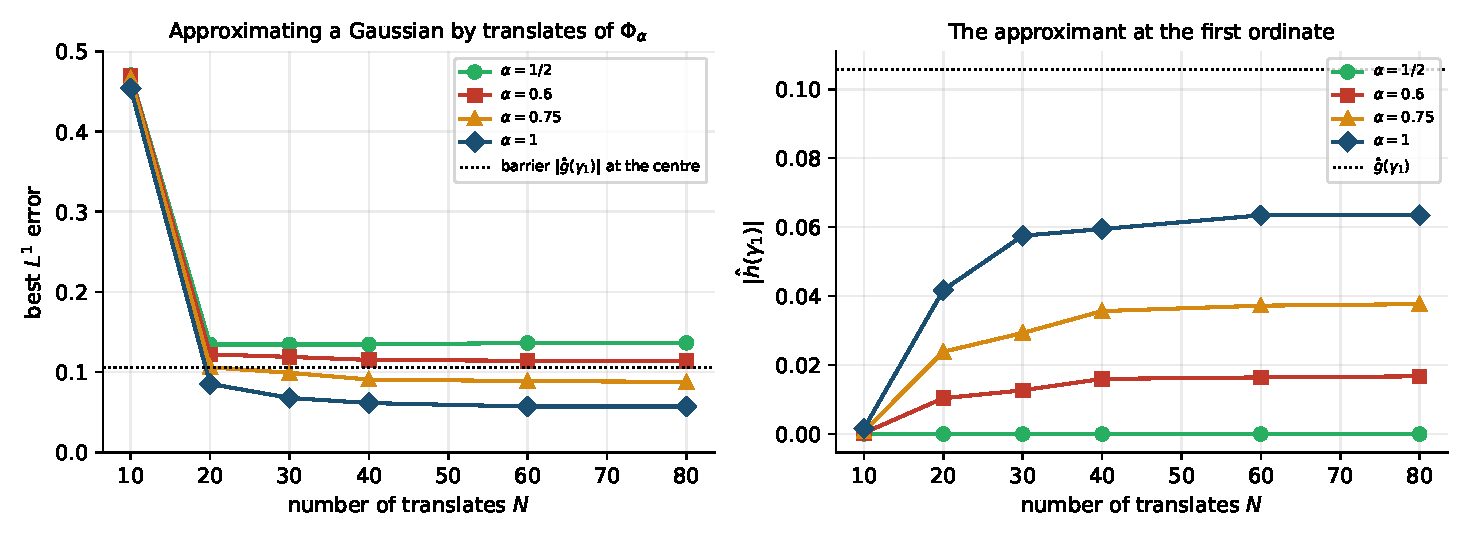
\includegraphics[width=\textwidth]{fig/bp1_wiener.pdf}
\caption{Left: best $L^1$ error against the number of translates, with the barrier at the centre. Right: the Fourier transform of the best approximant at the first ordinate, against the target $\hat g(\gamma_1)$. The data, which include $N=30$ and $N=60$, are in \texttt{wiener.json}, written by \texttt{wiener.py}, and \texttt{figs\_wiener.py} draws the figure.}
\label{wr:fig:wiener}
\end{figure}

\subsection{Salem's criterion and its P\'olya analogue}\label{wr:sec:salem}

Wiener's theorem has a dual form: for $k\in L^1(\R)$, the convolution equation $\int k(x-y)f(y)\,dy=0$ for all $x$ has a bounded solution $f\ne0$ if and only if $\hat k$ has a real zero, and then $f(y)=e^{-i\gamma y}$ is a solution for any real zero $\gamma$. Salem \cite{Salem53} used it to give one of the classical equivalents of RH: RH holds if and only if, for every $\frac12<\sigma<1$, the equation
\[
\int_{\R}\frac{e^{-\sigma y}f(y)}{e^{e^{x-y}}+1}\,dy=0\qquad(x\in\R)
\]
has no bounded solution other than $f=0$. Multiplied by $e^{\sigma x}$, it is the convolution equation with the kernel $k_\sigma(u)=e^{\sigma u}/(e^{e^u}+1)$, the Fermi Dirac function $1/(e^w+1)$ in the logarithmic variable $w=e^u$, and that substitution gives its Fourier transform,
\begin{gather*}
\hat k_\sigma(\theta)=\int_{\R}\frac{e^{\sigma u}e^{i\theta u}}{e^{e^u}+1}\,du=\int_0^\infty\frac{w^{\sigma+i\theta-1}}{e^w+1}\,dw=\Gamma(\sigma+i\theta)\,\eta(\sigma+i\theta),\\
\eta(s)=(1-2^{1-s})\zeta(s),
\end{gather*}
where $\eta$ is Dirichlet's alternating zeta function, not the Dedekind eta function of Section~\ref{ch:bpeta}. So for $\frac12<\sigma<1$ the real zeros of $\hat k_\sigma$ are exactly the ordinates of the zeros of $\zeta$ on the line $\re s=\sigma$, and Salem's criterion is Proposition~\ref{wr:prop:wiener}(4) with the Fermi Dirac kernel in place of the tilted P\'olya kernel \eqref{wr:eq:kernel}. Our family gives the P\'olya analogue directly.

\begin{corollary}\label{wr:cor:salem}
RH holds if and only if, for every $\frac12<\alpha<1$, the equation $\int_{\R}\Phi_\alpha(x-y)f(y)\,dy=0$ for all $x$ has no bounded solution $f\ne0$. At the centre the equation has the explicit bounded solutions $f(y)=\cos(\gamma y)$, one for each ordinate $\gamma$ of a zero on the critical line, because $\Xi(\gamma)=0$ there; at the basepoint one it has none.
\end{corollary}

\begin{proof}
By the dual form of Wiener's theorem with $k=\Phi_\alpha$, a bounded solution $f\ne0$ exists exactly when $\hat\Phi_\alpha(\theta)=\xi(\alpha+i\theta)$ has a real zero, that is, when $\zeta$ has a zero on the line $\re s=\alpha$. That no such zero exists for any $\alpha\in(\frac12,1)$ means that no zero has $\frac12<\re\rho<1$, which, since no zero lies on the line $\re s=1$, is RH by the symmetry $\rho\mapsto1-\rho$. At the centre $\Phi$ is even, so $\int_{\R}\Phi(x-y)\cos(\gamma y)\,dy=\Xi(\gamma)\cos(\gamma x)$, which vanishes when $\frac12+i\gamma$ is a zero; at the basepoint one $\xi(1+i\theta)\ne0$ for every real $\theta$.
\end{proof}

The two families differ at the edge of the strip. The factor $1-2^{1-s}$ in $\eta$ vanishes at $s=1+2\pi ik/\log2$ with $k\ne0$, so Salem's kernel has real Fourier zeros on the line $\sigma=1$, at $\theta=9.0647$, $18.1294$, $27.1942,\dots$, and its translates are not complete there, whereas the P\'olya family is complete at $\alpha=1$ because $\xi(1+i\theta)\ne0$. Inside the strip the two families have the same zeros and the criteria coincide. The left panel of Figure~\ref{wr:fig:salem}, computed by \texttt{salem\_riesz.py}, shows $|\eta(\sigma+i\theta)|$. At $\sigma=\frac12$ it dips to zero at every ordinate; at $\sigma=0.6$ the dips are shallow, the deepest on $(0,60]$ being $0.175$ near $\gamma_1$ and $0.189$ near $\gamma_6$; at $\sigma=0.75$ no dip goes below $0.2$; and at $\sigma=1$ the zeros of $1-2^{1-s}$ appear. The depth of the dips plays for Salem's kernel the role that $|\xi(\alpha+i\gamma)|$ plays in the cost of approximation of Proposition~\ref{wr:prop:wiener}(5), and it is of order $\sigma-\frac12$ near each ordinate.

\begin{figure}[htbp]
\centering
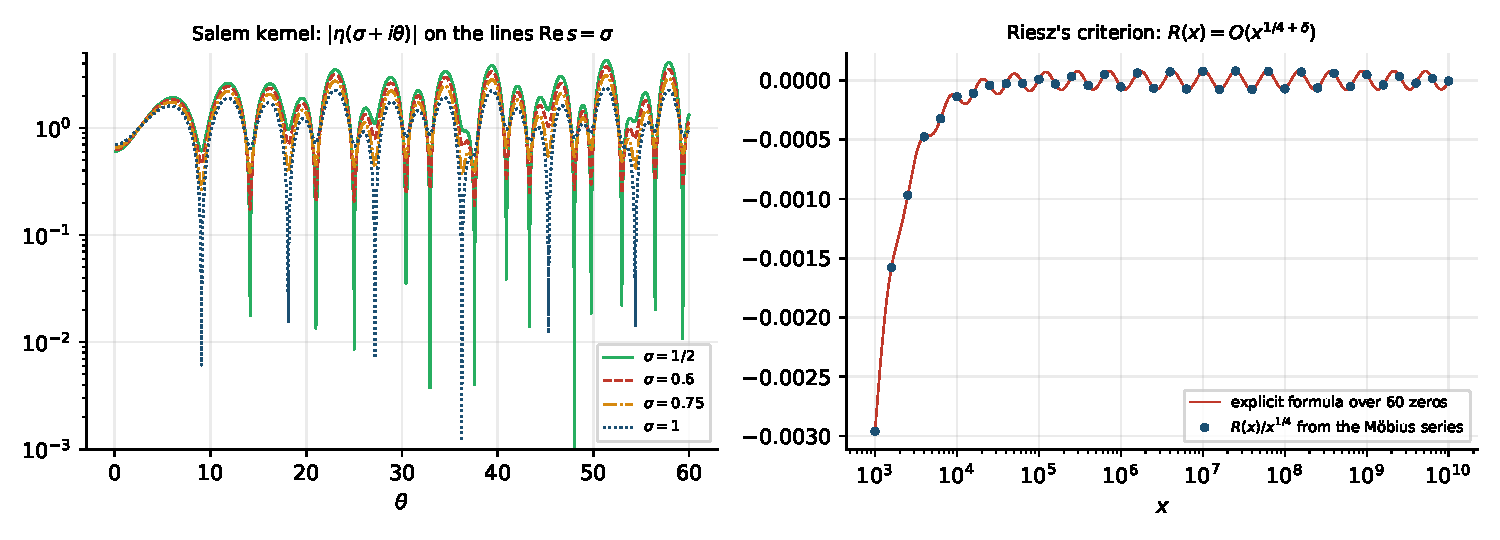
\includegraphics[width=\textwidth]{fig/bp1_salem_riesz.pdf}
\caption{Left: $|\eta(\sigma+i\theta)|$, the Fourier transform of Salem's kernel divided by $\Gamma(\sigma+i\theta)$, at $\sigma=\frac12$, $0.6$, $0.75$, $1$. Right: the Riesz function $R(x)/x^{1/4}$ from the M\"obius series and from the explicit formula \eqref{wr:eq:rieszexplicit} over $60$ zeros. The data are in \texttt{salem\_riesz.json}, written by \texttt{salem\_riesz.py}; \texttt{figs\_wiener.py} draws the figure and evaluates the explicit formula with the first $60$ ordinates in \texttt{g\_1\_400.npy} and the trivial terms in \texttt{riesz\_explicit.json}.}
\label{wr:fig:salem}
\end{figure}

\subsection{Riesz's criterion and multiplicative completeness}\label{wr:sec:riesz}

Riesz \cite{Riesz16} found the first criterion of this type, in terms of growth rather than completeness. With the M\"obius function $\mu(n)$, which is unrelated to the Thorin measure $\mu_\varepsilon$ of Section~\ref{ch:clock}, put
\begin{equation}\label{wr:eq:riesz}
R(x)=-\sum_{k\ge1}\frac{(-x)^k}{(k-1)!\,\zeta(2k)}=x\sum_{n\ge1}\frac{\mu(n)}{n^2}\,e^{-x/n^2},
\end{equation}
the second form following from $1/\zeta(2k)=\sum_n\mu(n)n^{-2k}$. Riesz proved that RH holds if and only if $R(x)=O(x^{1/4+\delta})$ for every $\delta>0$. The Mellin transform explains why: for $\frac12<\re s<1$,
\begin{equation}\label{wr:eq:rieszmellin}
\int_0^\infty R(x)\,x^{-s-1}dx=\frac{\Gamma(1-s)}{\zeta(2s)},
\end{equation}
whose poles in the strip $0<\re s<\frac12$ sit at $s=\rho/2$, and shifting the contour gives, when the zeros are simple, the explicit formula
\begin{equation}\label{wr:eq:rieszexplicit}
R(x)=\sum_\rho\frac{\Gamma(1-\rho/2)}{2\zeta'(\rho)}\,x^{\rho/2}+\sum_{k\ge1}\frac{\Gamma(1+k)}{2\zeta'(-2k)}\,x^{-k},
\end{equation}
in which the sum over the zeros is the limit of its partial sums over $|\gamma|<T_\nu$ along a suitable sequence of heights $T_\nu\to\infty$. The same argument gives the basepoint version: for $\frac12\le\alpha<1$, $\zeta$ has no zeros in $\re s>\alpha$ if and only if $R(x)=O(x^{\alpha/2+\delta})$ for every $\delta>0$. If the bound holds then, since also $|R(x)|\le\zeta(2)x$, the Mellin integral converges absolutely and is holomorphic on $\frac\alpha2<\re s<1$, so $\Gamma(1-s)/\zeta(2s)$ continues holomorphically there and $\zeta(w)\ne0$ for $\alpha<\re w<2$. Conversely, if $\zeta$ has no zeros in $\re s>\alpha$, the inversion integral $R(x)=\frac1{2\pi i}\int_{c-i\infty}^{c+i\infty}\Gamma(1-s)\zeta(2s)^{-1}x^s\,ds$, $\frac12<c<1$, moves to the line $\re s=\frac\alpha2+\delta$ without crossing a pole and gives $|R(x)|\le C_\delta x^{\alpha/2+\delta}$, provided $1/\zeta(\sigma+it)$ grows at most like a power of $|t|$ on $\sigma\ge\alpha+2\delta$, because $\Gamma(1-s)$ decays exponentially in vertical strips. The zero free half plane supplies that bound: the Borel Carath\'eodory lemma applied to $\log\zeta$ on discs centred at $2+it$ gives $\log\zeta(\sigma+it)=O_\delta(\log|t|)$ there, as in \cite[Section 14.2]{Titchmarsh} with the line $\re s=\alpha$ in place of the critical line; Proposition~\ref{ri:prop:twisted} carries out this argument in detail, for a twisted form of $R$. So Riesz's criterion runs through the same family of half planes as the constructions of Chapter~\ref{chap:basepoint}, with the growth exponent $\alpha/2$ in place of the basepoint.

In the language of this book, $R(x)/x=\sum_n\mu(n)n^{-2}e^{-x/n^2}$ is the Laplace transform of the signed M\"obius measure $\sum_n\mu(n)n^{-2}\delta_{1/n^2}$. It is a heat trace on the arithmetic side, with the M\"obius function in place of the zeros, and it is the same M\"obius series that underlies the representation of the reciprocal zeta function in Section~\ref{ch:rz1} (Theorem~\ref{rz:thm:sech}). Its sign carries no information; RH is encoded in its rate of growth, exactly as the zero free half planes are encoded in the growth of the error terms of Section~\ref{bp:sec:below}. The coefficients $1/\zeta(2k)$ of the power series of $R$ are, up to elementary factors, values of the Laplace transforms of the centre clock $T$ and of $T_1$ (Section~\ref{ri:sec:thorin}).

We computed $R(x)$ with \texttt{salem\_riesz.py} from the M\"obius series with $n\le N=10^7$, approximating
\[
R(x)\approx x\Big[\sum_{n\le N}\mu(n)n^{-2}\big(e^{-x/n^2}-1\big)+\frac6{\pi^2}\Big]
\]
to avoid the slowly converging tail, for $10\le x\le10^{12}$. Beyond $x\approx10^{10}$ the truncation at $N=10^7$ limits the accuracy: the omitted terms are about $-x^2\sum_{n>N}\mu(n)n^{-4}\approx9\times10^{-26}x^2$, that is $3\times10^{-8}$ in $R(x)/x^{1/4}$ at $x=10^{10}$ and $9\times10^{-5}$ at $x=10^{12}$. For $10^4\le x\le10^{10}$ the ratio $R(x)/x^{1/4}$ oscillates with amplitude about $1.1\times10^{-4}$, and for $10^5\le x\le10^{10}$ with amplitude $7.8\times10^{-5}$, which is the amplitude $|\Gamma(1-\rho_1/2)/\zeta'(\rho_1)|$ of the term of the first zero; the small constant reflects the decay of $\Gamma(1-\rho/2)$ along the critical line, which also makes the term of the second zero about $300$ times smaller. The larger swing near $x=10^4$ comes from the term $\Gamma(2)x^{-1}/(2\zeta'(-2))=-16.42\,x^{-1}$ of the first trivial zero, which contributes $-1.6\times10^{-4}$ to the ratio at $x=10^4$; the next two trivial zeros enter with the coefficients $\Gamma(1+k)/(2\zeta'(-2k))=125.25$ and $-508.50$ for $k=2$ and $3$. The explicit formula \eqref{wr:eq:rieszexplicit} with the first $60$ zeros and these three trivial terms reproduces the computed values to $3.1\times10^{-8}$ on $[10^3,10^{10}]$, against a signal of size up to $3\times10^{-3}$ (\texttt{riesz\_explicit.py}, output \texttt{riesz\_explicit.json}; Figure~\ref{wr:fig:salem}, right). The largest difference, at $x=10^{10}$, is the truncation error just described, and on $[10^3,10^9]$ the difference is at most $6.2\times10^{-10}$. The decay of $\Gamma(1-\rho/2)$ hides every zero above the first few from $R$. Section~\ref{ri:sec:filters} twists the M\"obius series by $(x/n^2)^{ih}$ so that it responds to the zeros near height $2h$, and computes $R$ to $x=10^{12}$ and its twists to $x=10^{10}$.

Wiener's theorem concerns translates. Its multiplicative counterpart concerns dilates, and there completeness is equivalent to RH itself. Nyman and Beurling \cite{Nyman50,Beurling55} proved that RH holds if and only if the constant function $1$ lies in the $L^2(0,1)$ closure of the span of the functions $r_\lambda(x)=\{\lambda/x\}-\lambda\{1/x\}$, $0<\lambda\le1$, where $\{\cdot\}$ is the fractional part, and B\'aez-Duarte \cite{BaezDuarte03} showed that $\lambda=1/n$ suffices. Under $x=e^{-u}$ this is a closure problem for translates in a weighted $L^2$ space on the half line, and the Mellin transform of $r_\lambda$ is $-\zeta(s)(\lambda^s-\lambda)/s$, so the zeros of $\zeta$ in the half plane $\re s>\frac12$ are exactly what obstructs the closure. The same framework governs the dilates $\sech(nx)$ of the Lai and Vere-Jones identity (Proposition~\ref{rz:prop:lvj}), which lies behind the expansion of Theorem~\ref{rz:thm:sech}: the Mellin transform of $\sech$ is $2\Gamma(s)L(s,\chi_4)$, and completeness of systems of dilates is controlled by where the associated Dirichlet series vanishes, in the sense of Beurling's periodic dilation problem and the work of Hedenmalm, Lindqvist and Seip \cite{HLS97}. How the two questions are related is the Nyman Beurling problem of Section~\ref{rz:sec:open}. Each of these completeness questions is by itself equivalent to RH or to the generalised Riemann hypothesis. The additive family of Proposition~\ref{wr:prop:wiener} is the probabilistic one, and it reaches RH only as $\alpha\downarrow\frac12$, in the same way as every other construction of Chapters~\ref{chap:basepoint} to \ref{chap:almost}.

The normal scale mixtures of this section are Brownian motion run at the clock $2T_\alpha$, and their classes are read off those of $T_\alpha$: infinite divisibility holds with no hypothesis, and the EGGC property holds exactly when $T_\alpha$ is a GGC. The completeness statements are the same zero free half planes read through Fourier transforms, and Riesz's criterion reads them through the growth of $R(x)$. Section~\ref{ch:riesz} takes up that criterion.
